% =============================================================================
% 02-algorithm-analysis-notes.tex — Lecture Notes for Week 2:
% What Does an Operation Cost? Running Time, Asymptotic Notation, and
% Best/Worst/Average Case
%
% DERIVED ARTIFACT. Source of truth: Slides/CS301/02-algorithm-analysis.tex.
% Generated by /lecture-notes at the "textbook-candidate prose" Detail Bar
% (every trace step written out, every example fully solved, Exercises with a
% separate Solutions block, reading guidance per section); do not hand-edit
% content independently of the Beamer source without re-running /qa-notes
% afterward (single-source-of-truth.md).
%
% Page-verified anchors (per knowledge-base-CS301.md /
% master_supporting_docs/CS301/supporting_books/Sedgewick2011/index.md):
%   Sedgewick2011: p.172 (S1.4 opener) -- "how long will my program take"
%   motivating question; p.187 (S1.4, order-of-growth classification table).
% Karumanchi2017 is cited at chapter level only (Ch.1, pp.16-61 PDF; no
% page-verified spot anchor exists yet for the best/worst/average-case
% content specifically). Horowitz & Sahni Ch.1 and Neapolitan & Naimipour
% Ch.1-2 are chapter-level only (not yet page-indexed), matching the deck's
% own citation precision -- no page number is invented for any of these
% three per textbook-grounding.md.
%
% Compile with (Windows/MiKTeX, ';'-joined TEXINPUTS/BIBINPUTS): cd Notes/CS301 &&
%   TEXINPUTS="../../Preambles;" xelatex -interaction=nonstopmode 02-algorithm-analysis-notes.tex
%   BIBINPUTS="../..;" bibtex 02-algorithm-analysis-notes
%   TEXINPUTS="../../Preambles;" xelatex -interaction=nonstopmode 02-algorithm-analysis-notes.tex  (x2)
% =============================================================================

\documentclass[11pt]{article}
\usepackage[margin=1in]{geometry}
% =============================================================================
% Preambles/header.tex — shared LaTeX/Beamer preamble for this project
%
% Use from a Beamer lecture by prepending:
%     % =============================================================================
% Preambles/header.tex — shared LaTeX/Beamer preamble for this project
%
% Use from a Beamer lecture by prepending:
%     % =============================================================================
% Preambles/header.tex — shared LaTeX/Beamer preamble for this project
%
% Use from a Beamer lecture by prepending:
%     \input{header}
% and compiling with TEXINPUTS=../Preambles:$TEXINPUTS (the /compile-latex
% skill does this automatically).
%
% PALETTE CONTRACT. Color names defined here MUST match the names in
% Quarto/theme-template.scss so Beamer and Quarto renderings use the same
% palette. The scripts/check-palette-sync.sh script enforces this.
%
% To customize: edit the HEX values below AND the matching $variable in
% Quarto/theme-template.scss, then run scripts/check-palette-sync.sh.
%
% TITLE PAGE. A formal, serif (Libertine) title-page template is defined in
% the Beamer-only block below (\setbeamertemplate{title page}) -- title,
% subtitle, a thin gold rule, then \author/\institute/\date. Frametitle and
% body text remain on Beamer's sans-serif default. No SCSS counterpart is
% needed for this (font/layout only, no new colors).
% =============================================================================

% -----------------------------------------------------------------------------
% Engine detection + encoding
%
% Our /compile-latex skill uses XeLaTeX, where inputenc is unnecessary and
% can produce encoding warnings. Only load inputenc under pdfTeX.
% -----------------------------------------------------------------------------
\usepackage{iftex}
\ifPDFTeX
  \usepackage[utf8]{inputenc}
\fi

\usepackage{amsmath, amssymb, amsthm}
\usepackage{booktabs}
\usepackage{graphicx}

% -----------------------------------------------------------------------------
% Serif face for the title page (formal/academic look). Linux Libertine is
% XeLaTeX- and pdfTeX-safe and redefines \rmdefault, so \rmfamily picks it up
% everywhere \rmfamily is used explicitly. Body text and frametitles stay on
% Beamer's own sans-serif default (unaffected) -- only the title-page
% \setbeamerfont{...} overrides below opt in to \rmfamily.
% -----------------------------------------------------------------------------
\usepackage{libertine}

% -----------------------------------------------------------------------------
% PALETTE — mirrors Quarto/theme-template.scss variable names.
% Load xcolor and define colors BEFORE anything that references them
% (notably hyperref, hypersetup, and the Beamer color assignments).
% -----------------------------------------------------------------------------
\usepackage{xcolor}

\definecolor{primary-blue}{HTML}{012169}      % headings, accents
\definecolor{primary-gold}{HTML}{B9975B}      % emphasis, borders
\definecolor{highlight-yellow}{HTML}{F2A900}  % markers, alerts
\definecolor{light-bg}{HTML}{E8EDF5}          % title / section backgrounds
\definecolor{jet}{HTML}{1A1A1A}               % body text

% Semantic colors (used in diagrams and annotations)
\definecolor{positive}{HTML}{15803D}          % good / observed / identified
\definecolor{negative}{HTML}{B91C1C}          % bad / problematic / bias
\definecolor{neutral}{HTML}{525252}           % reference / context

% Highlight accents (match .hi-* classes in the SCSS)
\definecolor{hi-slate}{HTML}{314F4F}
\definecolor{hi-green}{HTML}{2E8B57}
\definecolor{hi-red}{HTML}{C41E3A}

% Semantic aliases so skill templates and snippets can write
% \textcolor{accent}{...} without hard-coding "primary-blue".
\colorlet{accent}{primary-blue}
\colorlet{accent2}{primary-gold}

% -----------------------------------------------------------------------------
% Hyperref — loaded AFTER xcolor + palette so link colors resolve.
% -----------------------------------------------------------------------------
\usepackage{hyperref}
\hypersetup{colorlinks=true, linkcolor=primary-blue, urlcolor=primary-blue,
            citecolor=primary-blue, pdfborder={0 0 0}}

% -----------------------------------------------------------------------------
% Course code — set once per deck (after \input{header}, before \begin{document})
% via \coursecode{CS401}. Shown in the footer on every slide so a deck's course
% is identifiable without opening the title page. Empty by default.
% -----------------------------------------------------------------------------
\makeatletter
\newcommand{\coursecode}[1]{\gdef\@coursecodetext{#1}}
\gdef\@coursecodetext{}
\makeatother

% -----------------------------------------------------------------------------
% Beamer theme assignments (only apply under Beamer).
%
% We detect Beamer via \@ifclassloaded{beamer}, which is the documented,
% non-internal way. This must be wrapped in \makeatletter/\makeatother
% because \@ifclassloaded contains an @-catcode character.
% -----------------------------------------------------------------------------
\makeatletter
\@ifclassloaded{beamer}{%
  \usefonttheme{professionalfonts}
  \setbeamercolor{structure}{fg=primary-blue}
  \setbeamercolor{frametitle}{fg=primary-blue}
  \setbeamercolor{title}{fg=primary-blue}
  \setbeamercolor{subtitle}{fg=primary-gold}
  \setbeamercolor{author}{fg=primary-blue}
  \setbeamercolor{institute}{fg=neutral}
  \setbeamercolor{date}{fg=primary-gold}
  \setbeamercolor{itemize item}{fg=primary-blue}
  \setbeamercolor{itemize subitem}{fg=primary-gold}
  \setbeamercolor{alerted text}{fg=primary-gold}
  \setbeamercolor{block title}{fg=white, bg=primary-blue}
  \setbeamercolor{block body}{bg=light-bg}
  % Semantic block variants: block=definition/concept (blue), exampleblock=
  % worked example (green/positive), alertblock=key takeaway or caution (gold).
  % Keep to <=2 colored boxes per slide across ALL three variants (INV-7).
  \setbeamercolor{block title example}{fg=white, bg=positive}
  \setbeamercolor{block body example}{bg=light-bg}
  \setbeamercolor{block title alerted}{fg=white, bg=primary-gold}
  \setbeamercolor{block body alerted}{bg=light-bg}

  % ---------------------------------------------------------------------------
  % Formal title page: serif (Libertine, via \rmfamily) for title-page
  % elements only. Body text, itemize, and frametitle are intentionally left
  % on Beamer's sans-serif default -- \usebeamerfont{title} is also what
  % \transitionslide (below) uses for its big centered text, so section
  % transitions pick up the same serif treatment for free.
  % ---------------------------------------------------------------------------
  \setbeamerfont{title}{family=\rmfamily, series=\bfseries, size=\Large}
  \setbeamerfont{subtitle}{family=\rmfamily, shape=\itshape, size=\normalsize}
  \setbeamerfont{author}{family=\rmfamily, size=\normalsize}
  \setbeamerfont{institute}{family=\rmfamily, size=\scriptsize}
  \setbeamerfont{date}{family=\rmfamily, size=\scriptsize}

  \setbeamertemplate{title page}{
    \vfill
    \begin{center}
      {\usebeamerfont{title}\usebeamercolor[fg]{title}\inserttitle\par}
      \vspace{0.15cm}
      {\usebeamerfont{subtitle}\usebeamercolor[fg]{subtitle}\insertsubtitle\par}
      \vspace{0.45cm}
      {\color{primary-gold}\rule{0.42\textwidth}{0.6pt}\par}
      \vspace{0.45cm}
      {\usebeamerfont{author}\usebeamercolor[fg]{author}\insertauthor\par}
      \vspace{0.35cm}
      {\usebeamerfont{institute}\usebeamercolor[fg]{institute}\insertinstitute\par}
      \vspace{0.35cm}
      {\usebeamerfont{date}\usebeamercolor[fg]{date}\insertdate\par}
    \end{center}
    \vfill
  }

  % Minimal footer: course code (left) + page X / N (right), no navigation clutter
  \setbeamertemplate{navigation symbols}{}
  \setbeamertemplate{footline}{%
    \color{neutral}\footnotesize\hspace{0.7em}\@coursecodetext\hfill
    \insertframenumber/\inserttotalframenumber\hspace{0.7em}\vspace{0.3em}}
}{}
\makeatother

% -----------------------------------------------------------------------------
% TikZ setup — libraries the snippet gallery uses
% -----------------------------------------------------------------------------
\usepackage{tikz}
\usetikzlibrary{arrows.meta, positioning, calc, decorations.pathreplacing,
                fit, shapes.geometric, backgrounds}

% Shared TikZ styles — snippets and hand-written diagrams can pick these up
% via `\begin{tikzpicture}[every node/.style={...}]` or by naming specific
% styles (e.g., `\node[dag-node] (X) at (0,0) {X};`).
\tikzset{
  % Node styles for causal DAGs and similar
  dag-node/.style = {
    draw=primary-blue, fill=light-bg, rounded corners=2pt,
    minimum width=1.2cm, minimum height=0.9cm, align=center, font=\small
  },
  decision-node/.style = {
    draw=primary-gold, fill=white, diamond, aspect=1.8,
    minimum width=1.8cm, minimum height=1.2cm, align=center, font=\small,
    inner sep=1pt
  },
  % Edge styles — observed vs counterfactual
  observed-edge/.style = {-{Latex[length=2.5mm]}, thick, draw=jet},
  counterfactual-edge/.style = {-{Latex[length=2.5mm]}, thick, draw=neutral, dashed},
  confound-edge/.style = {-{Latex[length=2.5mm]}, thick, draw=negative, dashed},
  % Data-point styles for plots
  observed-dot/.style = {fill=primary-blue, draw=primary-blue, circle, inner sep=1.2pt},
  counterfactual-dot/.style = {fill=white, draw=neutral, circle, inner sep=1.2pt}
}

% -----------------------------------------------------------------------------
% Convenience macros
% -----------------------------------------------------------------------------
\newcommand{\muted}[1]{\textcolor{neutral}{#1}}
\newcommand{\key}[1]{\textcolor{primary-gold}{\textbf{#1}}}
\newcommand{\good}[1]{\textcolor{positive}{#1}}
\newcommand{\bad}[1]{\textcolor{negative}{#1}}

% Standout frame macro: full-bleed dark background for section transitions.
% Beamer-only (uses \begin{frame}/\setbeamercolor/\usebeamerfont) -- do not
% call from an article-class file (e.g. Notes/<CODE>/*-notes.tex). \muted,
% \key, \good, \bad, and \coursecode above are plain xcolor/gdef and are
% safe to use from either class; verified when Notes/article-class support
% was added.
% Expand: \transitionslide{Your transition title}
\newcommand{\transitionslide}[1]{%
  \begingroup
  \setbeamercolor{background canvas}{bg=primary-blue}
  \begin{frame}[plain]
    \centering
    \vfill
    {\usebeamerfont{title}\color{white}\Large #1\par}
    \vfill
  \end{frame}
  \endgroup
}

% and compiling with TEXINPUTS=../Preambles:$TEXINPUTS (the /compile-latex
% skill does this automatically).
%
% PALETTE CONTRACT. Color names defined here MUST match the names in
% Quarto/theme-template.scss so Beamer and Quarto renderings use the same
% palette. The scripts/check-palette-sync.sh script enforces this.
%
% To customize: edit the HEX values below AND the matching $variable in
% Quarto/theme-template.scss, then run scripts/check-palette-sync.sh.
%
% TITLE PAGE. A formal, serif (Libertine) title-page template is defined in
% the Beamer-only block below (\setbeamertemplate{title page}) -- title,
% subtitle, a thin gold rule, then \author/\institute/\date. Frametitle and
% body text remain on Beamer's sans-serif default. No SCSS counterpart is
% needed for this (font/layout only, no new colors).
% =============================================================================

% -----------------------------------------------------------------------------
% Engine detection + encoding
%
% Our /compile-latex skill uses XeLaTeX, where inputenc is unnecessary and
% can produce encoding warnings. Only load inputenc under pdfTeX.
% -----------------------------------------------------------------------------
\usepackage{iftex}
\ifPDFTeX
  \usepackage[utf8]{inputenc}
\fi

\usepackage{amsmath, amssymb, amsthm}
\usepackage{booktabs}
\usepackage{graphicx}

% -----------------------------------------------------------------------------
% Serif face for the title page (formal/academic look). Linux Libertine is
% XeLaTeX- and pdfTeX-safe and redefines \rmdefault, so \rmfamily picks it up
% everywhere \rmfamily is used explicitly. Body text and frametitles stay on
% Beamer's own sans-serif default (unaffected) -- only the title-page
% \setbeamerfont{...} overrides below opt in to \rmfamily.
% -----------------------------------------------------------------------------
\usepackage{libertine}

% -----------------------------------------------------------------------------
% PALETTE — mirrors Quarto/theme-template.scss variable names.
% Load xcolor and define colors BEFORE anything that references them
% (notably hyperref, hypersetup, and the Beamer color assignments).
% -----------------------------------------------------------------------------
\usepackage{xcolor}

\definecolor{primary-blue}{HTML}{012169}      % headings, accents
\definecolor{primary-gold}{HTML}{B9975B}      % emphasis, borders
\definecolor{highlight-yellow}{HTML}{F2A900}  % markers, alerts
\definecolor{light-bg}{HTML}{E8EDF5}          % title / section backgrounds
\definecolor{jet}{HTML}{1A1A1A}               % body text

% Semantic colors (used in diagrams and annotations)
\definecolor{positive}{HTML}{15803D}          % good / observed / identified
\definecolor{negative}{HTML}{B91C1C}          % bad / problematic / bias
\definecolor{neutral}{HTML}{525252}           % reference / context

% Highlight accents (match .hi-* classes in the SCSS)
\definecolor{hi-slate}{HTML}{314F4F}
\definecolor{hi-green}{HTML}{2E8B57}
\definecolor{hi-red}{HTML}{C41E3A}

% Semantic aliases so skill templates and snippets can write
% \textcolor{accent}{...} without hard-coding "primary-blue".
\colorlet{accent}{primary-blue}
\colorlet{accent2}{primary-gold}

% -----------------------------------------------------------------------------
% Hyperref — loaded AFTER xcolor + palette so link colors resolve.
% -----------------------------------------------------------------------------
\usepackage{hyperref}
\hypersetup{colorlinks=true, linkcolor=primary-blue, urlcolor=primary-blue,
            citecolor=primary-blue, pdfborder={0 0 0}}

% -----------------------------------------------------------------------------
% Course code — set once per deck (after % =============================================================================
% Preambles/header.tex — shared LaTeX/Beamer preamble for this project
%
% Use from a Beamer lecture by prepending:
%     \input{header}
% and compiling with TEXINPUTS=../Preambles:$TEXINPUTS (the /compile-latex
% skill does this automatically).
%
% PALETTE CONTRACT. Color names defined here MUST match the names in
% Quarto/theme-template.scss so Beamer and Quarto renderings use the same
% palette. The scripts/check-palette-sync.sh script enforces this.
%
% To customize: edit the HEX values below AND the matching $variable in
% Quarto/theme-template.scss, then run scripts/check-palette-sync.sh.
%
% TITLE PAGE. A formal, serif (Libertine) title-page template is defined in
% the Beamer-only block below (\setbeamertemplate{title page}) -- title,
% subtitle, a thin gold rule, then \author/\institute/\date. Frametitle and
% body text remain on Beamer's sans-serif default. No SCSS counterpart is
% needed for this (font/layout only, no new colors).
% =============================================================================

% -----------------------------------------------------------------------------
% Engine detection + encoding
%
% Our /compile-latex skill uses XeLaTeX, where inputenc is unnecessary and
% can produce encoding warnings. Only load inputenc under pdfTeX.
% -----------------------------------------------------------------------------
\usepackage{iftex}
\ifPDFTeX
  \usepackage[utf8]{inputenc}
\fi

\usepackage{amsmath, amssymb, amsthm}
\usepackage{booktabs}
\usepackage{graphicx}

% -----------------------------------------------------------------------------
% Serif face for the title page (formal/academic look). Linux Libertine is
% XeLaTeX- and pdfTeX-safe and redefines \rmdefault, so \rmfamily picks it up
% everywhere \rmfamily is used explicitly. Body text and frametitles stay on
% Beamer's own sans-serif default (unaffected) -- only the title-page
% \setbeamerfont{...} overrides below opt in to \rmfamily.
% -----------------------------------------------------------------------------
\usepackage{libertine}

% -----------------------------------------------------------------------------
% PALETTE — mirrors Quarto/theme-template.scss variable names.
% Load xcolor and define colors BEFORE anything that references them
% (notably hyperref, hypersetup, and the Beamer color assignments).
% -----------------------------------------------------------------------------
\usepackage{xcolor}

\definecolor{primary-blue}{HTML}{012169}      % headings, accents
\definecolor{primary-gold}{HTML}{B9975B}      % emphasis, borders
\definecolor{highlight-yellow}{HTML}{F2A900}  % markers, alerts
\definecolor{light-bg}{HTML}{E8EDF5}          % title / section backgrounds
\definecolor{jet}{HTML}{1A1A1A}               % body text

% Semantic colors (used in diagrams and annotations)
\definecolor{positive}{HTML}{15803D}          % good / observed / identified
\definecolor{negative}{HTML}{B91C1C}          % bad / problematic / bias
\definecolor{neutral}{HTML}{525252}           % reference / context

% Highlight accents (match .hi-* classes in the SCSS)
\definecolor{hi-slate}{HTML}{314F4F}
\definecolor{hi-green}{HTML}{2E8B57}
\definecolor{hi-red}{HTML}{C41E3A}

% Semantic aliases so skill templates and snippets can write
% \textcolor{accent}{...} without hard-coding "primary-blue".
\colorlet{accent}{primary-blue}
\colorlet{accent2}{primary-gold}

% -----------------------------------------------------------------------------
% Hyperref — loaded AFTER xcolor + palette so link colors resolve.
% -----------------------------------------------------------------------------
\usepackage{hyperref}
\hypersetup{colorlinks=true, linkcolor=primary-blue, urlcolor=primary-blue,
            citecolor=primary-blue, pdfborder={0 0 0}}

% -----------------------------------------------------------------------------
% Course code — set once per deck (after \input{header}, before \begin{document})
% via \coursecode{CS401}. Shown in the footer on every slide so a deck's course
% is identifiable without opening the title page. Empty by default.
% -----------------------------------------------------------------------------
\makeatletter
\newcommand{\coursecode}[1]{\gdef\@coursecodetext{#1}}
\gdef\@coursecodetext{}
\makeatother

% -----------------------------------------------------------------------------
% Beamer theme assignments (only apply under Beamer).
%
% We detect Beamer via \@ifclassloaded{beamer}, which is the documented,
% non-internal way. This must be wrapped in \makeatletter/\makeatother
% because \@ifclassloaded contains an @-catcode character.
% -----------------------------------------------------------------------------
\makeatletter
\@ifclassloaded{beamer}{%
  \usefonttheme{professionalfonts}
  \setbeamercolor{structure}{fg=primary-blue}
  \setbeamercolor{frametitle}{fg=primary-blue}
  \setbeamercolor{title}{fg=primary-blue}
  \setbeamercolor{subtitle}{fg=primary-gold}
  \setbeamercolor{author}{fg=primary-blue}
  \setbeamercolor{institute}{fg=neutral}
  \setbeamercolor{date}{fg=primary-gold}
  \setbeamercolor{itemize item}{fg=primary-blue}
  \setbeamercolor{itemize subitem}{fg=primary-gold}
  \setbeamercolor{alerted text}{fg=primary-gold}
  \setbeamercolor{block title}{fg=white, bg=primary-blue}
  \setbeamercolor{block body}{bg=light-bg}
  % Semantic block variants: block=definition/concept (blue), exampleblock=
  % worked example (green/positive), alertblock=key takeaway or caution (gold).
  % Keep to <=2 colored boxes per slide across ALL three variants (INV-7).
  \setbeamercolor{block title example}{fg=white, bg=positive}
  \setbeamercolor{block body example}{bg=light-bg}
  \setbeamercolor{block title alerted}{fg=white, bg=primary-gold}
  \setbeamercolor{block body alerted}{bg=light-bg}

  % ---------------------------------------------------------------------------
  % Formal title page: serif (Libertine, via \rmfamily) for title-page
  % elements only. Body text, itemize, and frametitle are intentionally left
  % on Beamer's sans-serif default -- \usebeamerfont{title} is also what
  % \transitionslide (below) uses for its big centered text, so section
  % transitions pick up the same serif treatment for free.
  % ---------------------------------------------------------------------------
  \setbeamerfont{title}{family=\rmfamily, series=\bfseries, size=\Large}
  \setbeamerfont{subtitle}{family=\rmfamily, shape=\itshape, size=\normalsize}
  \setbeamerfont{author}{family=\rmfamily, size=\normalsize}
  \setbeamerfont{institute}{family=\rmfamily, size=\scriptsize}
  \setbeamerfont{date}{family=\rmfamily, size=\scriptsize}

  \setbeamertemplate{title page}{
    \vfill
    \begin{center}
      {\usebeamerfont{title}\usebeamercolor[fg]{title}\inserttitle\par}
      \vspace{0.15cm}
      {\usebeamerfont{subtitle}\usebeamercolor[fg]{subtitle}\insertsubtitle\par}
      \vspace{0.45cm}
      {\color{primary-gold}\rule{0.42\textwidth}{0.6pt}\par}
      \vspace{0.45cm}
      {\usebeamerfont{author}\usebeamercolor[fg]{author}\insertauthor\par}
      \vspace{0.35cm}
      {\usebeamerfont{institute}\usebeamercolor[fg]{institute}\insertinstitute\par}
      \vspace{0.35cm}
      {\usebeamerfont{date}\usebeamercolor[fg]{date}\insertdate\par}
    \end{center}
    \vfill
  }

  % Minimal footer: course code (left) + page X / N (right), no navigation clutter
  \setbeamertemplate{navigation symbols}{}
  \setbeamertemplate{footline}{%
    \color{neutral}\footnotesize\hspace{0.7em}\@coursecodetext\hfill
    \insertframenumber/\inserttotalframenumber\hspace{0.7em}\vspace{0.3em}}
}{}
\makeatother

% -----------------------------------------------------------------------------
% TikZ setup — libraries the snippet gallery uses
% -----------------------------------------------------------------------------
\usepackage{tikz}
\usetikzlibrary{arrows.meta, positioning, calc, decorations.pathreplacing,
                fit, shapes.geometric, backgrounds}

% Shared TikZ styles — snippets and hand-written diagrams can pick these up
% via `\begin{tikzpicture}[every node/.style={...}]` or by naming specific
% styles (e.g., `\node[dag-node] (X) at (0,0) {X};`).
\tikzset{
  % Node styles for causal DAGs and similar
  dag-node/.style = {
    draw=primary-blue, fill=light-bg, rounded corners=2pt,
    minimum width=1.2cm, minimum height=0.9cm, align=center, font=\small
  },
  decision-node/.style = {
    draw=primary-gold, fill=white, diamond, aspect=1.8,
    minimum width=1.8cm, minimum height=1.2cm, align=center, font=\small,
    inner sep=1pt
  },
  % Edge styles — observed vs counterfactual
  observed-edge/.style = {-{Latex[length=2.5mm]}, thick, draw=jet},
  counterfactual-edge/.style = {-{Latex[length=2.5mm]}, thick, draw=neutral, dashed},
  confound-edge/.style = {-{Latex[length=2.5mm]}, thick, draw=negative, dashed},
  % Data-point styles for plots
  observed-dot/.style = {fill=primary-blue, draw=primary-blue, circle, inner sep=1.2pt},
  counterfactual-dot/.style = {fill=white, draw=neutral, circle, inner sep=1.2pt}
}

% -----------------------------------------------------------------------------
% Convenience macros
% -----------------------------------------------------------------------------
\newcommand{\muted}[1]{\textcolor{neutral}{#1}}
\newcommand{\key}[1]{\textcolor{primary-gold}{\textbf{#1}}}
\newcommand{\good}[1]{\textcolor{positive}{#1}}
\newcommand{\bad}[1]{\textcolor{negative}{#1}}

% Standout frame macro: full-bleed dark background for section transitions.
% Beamer-only (uses \begin{frame}/\setbeamercolor/\usebeamerfont) -- do not
% call from an article-class file (e.g. Notes/<CODE>/*-notes.tex). \muted,
% \key, \good, \bad, and \coursecode above are plain xcolor/gdef and are
% safe to use from either class; verified when Notes/article-class support
% was added.
% Expand: \transitionslide{Your transition title}
\newcommand{\transitionslide}[1]{%
  \begingroup
  \setbeamercolor{background canvas}{bg=primary-blue}
  \begin{frame}[plain]
    \centering
    \vfill
    {\usebeamerfont{title}\color{white}\Large #1\par}
    \vfill
  \end{frame}
  \endgroup
}
, before \begin{document})
% via \coursecode{CS401}. Shown in the footer on every slide so a deck's course
% is identifiable without opening the title page. Empty by default.
% -----------------------------------------------------------------------------
\makeatletter
\newcommand{\coursecode}[1]{\gdef\@coursecodetext{#1}}
\gdef\@coursecodetext{}
\makeatother

% -----------------------------------------------------------------------------
% Beamer theme assignments (only apply under Beamer).
%
% We detect Beamer via \@ifclassloaded{beamer}, which is the documented,
% non-internal way. This must be wrapped in \makeatletter/\makeatother
% because \@ifclassloaded contains an @-catcode character.
% -----------------------------------------------------------------------------
\makeatletter
\@ifclassloaded{beamer}{%
  \usefonttheme{professionalfonts}
  \setbeamercolor{structure}{fg=primary-blue}
  \setbeamercolor{frametitle}{fg=primary-blue}
  \setbeamercolor{title}{fg=primary-blue}
  \setbeamercolor{subtitle}{fg=primary-gold}
  \setbeamercolor{author}{fg=primary-blue}
  \setbeamercolor{institute}{fg=neutral}
  \setbeamercolor{date}{fg=primary-gold}
  \setbeamercolor{itemize item}{fg=primary-blue}
  \setbeamercolor{itemize subitem}{fg=primary-gold}
  \setbeamercolor{alerted text}{fg=primary-gold}
  \setbeamercolor{block title}{fg=white, bg=primary-blue}
  \setbeamercolor{block body}{bg=light-bg}
  % Semantic block variants: block=definition/concept (blue), exampleblock=
  % worked example (green/positive), alertblock=key takeaway or caution (gold).
  % Keep to <=2 colored boxes per slide across ALL three variants (INV-7).
  \setbeamercolor{block title example}{fg=white, bg=positive}
  \setbeamercolor{block body example}{bg=light-bg}
  \setbeamercolor{block title alerted}{fg=white, bg=primary-gold}
  \setbeamercolor{block body alerted}{bg=light-bg}

  % ---------------------------------------------------------------------------
  % Formal title page: serif (Libertine, via \rmfamily) for title-page
  % elements only. Body text, itemize, and frametitle are intentionally left
  % on Beamer's sans-serif default -- \usebeamerfont{title} is also what
  % \transitionslide (below) uses for its big centered text, so section
  % transitions pick up the same serif treatment for free.
  % ---------------------------------------------------------------------------
  \setbeamerfont{title}{family=\rmfamily, series=\bfseries, size=\Large}
  \setbeamerfont{subtitle}{family=\rmfamily, shape=\itshape, size=\normalsize}
  \setbeamerfont{author}{family=\rmfamily, size=\normalsize}
  \setbeamerfont{institute}{family=\rmfamily, size=\scriptsize}
  \setbeamerfont{date}{family=\rmfamily, size=\scriptsize}

  \setbeamertemplate{title page}{
    \vfill
    \begin{center}
      {\usebeamerfont{title}\usebeamercolor[fg]{title}\inserttitle\par}
      \vspace{0.15cm}
      {\usebeamerfont{subtitle}\usebeamercolor[fg]{subtitle}\insertsubtitle\par}
      \vspace{0.45cm}
      {\color{primary-gold}\rule{0.42\textwidth}{0.6pt}\par}
      \vspace{0.45cm}
      {\usebeamerfont{author}\usebeamercolor[fg]{author}\insertauthor\par}
      \vspace{0.35cm}
      {\usebeamerfont{institute}\usebeamercolor[fg]{institute}\insertinstitute\par}
      \vspace{0.35cm}
      {\usebeamerfont{date}\usebeamercolor[fg]{date}\insertdate\par}
    \end{center}
    \vfill
  }

  % Minimal footer: course code (left) + page X / N (right), no navigation clutter
  \setbeamertemplate{navigation symbols}{}
  \setbeamertemplate{footline}{%
    \color{neutral}\footnotesize\hspace{0.7em}\@coursecodetext\hfill
    \insertframenumber/\inserttotalframenumber\hspace{0.7em}\vspace{0.3em}}
}{}
\makeatother

% -----------------------------------------------------------------------------
% TikZ setup — libraries the snippet gallery uses
% -----------------------------------------------------------------------------
\usepackage{tikz}
\usetikzlibrary{arrows.meta, positioning, calc, decorations.pathreplacing,
                fit, shapes.geometric, backgrounds}

% Shared TikZ styles — snippets and hand-written diagrams can pick these up
% via `\begin{tikzpicture}[every node/.style={...}]` or by naming specific
% styles (e.g., `\node[dag-node] (X) at (0,0) {X};`).
\tikzset{
  % Node styles for causal DAGs and similar
  dag-node/.style = {
    draw=primary-blue, fill=light-bg, rounded corners=2pt,
    minimum width=1.2cm, minimum height=0.9cm, align=center, font=\small
  },
  decision-node/.style = {
    draw=primary-gold, fill=white, diamond, aspect=1.8,
    minimum width=1.8cm, minimum height=1.2cm, align=center, font=\small,
    inner sep=1pt
  },
  % Edge styles — observed vs counterfactual
  observed-edge/.style = {-{Latex[length=2.5mm]}, thick, draw=jet},
  counterfactual-edge/.style = {-{Latex[length=2.5mm]}, thick, draw=neutral, dashed},
  confound-edge/.style = {-{Latex[length=2.5mm]}, thick, draw=negative, dashed},
  % Data-point styles for plots
  observed-dot/.style = {fill=primary-blue, draw=primary-blue, circle, inner sep=1.2pt},
  counterfactual-dot/.style = {fill=white, draw=neutral, circle, inner sep=1.2pt}
}

% -----------------------------------------------------------------------------
% Convenience macros
% -----------------------------------------------------------------------------
\newcommand{\muted}[1]{\textcolor{neutral}{#1}}
\newcommand{\key}[1]{\textcolor{primary-gold}{\textbf{#1}}}
\newcommand{\good}[1]{\textcolor{positive}{#1}}
\newcommand{\bad}[1]{\textcolor{negative}{#1}}

% Standout frame macro: full-bleed dark background for section transitions.
% Beamer-only (uses \begin{frame}/\setbeamercolor/\usebeamerfont) -- do not
% call from an article-class file (e.g. Notes/<CODE>/*-notes.tex). \muted,
% \key, \good, \bad, and \coursecode above are plain xcolor/gdef and are
% safe to use from either class; verified when Notes/article-class support
% was added.
% Expand: \transitionslide{Your transition title}
\newcommand{\transitionslide}[1]{%
  \begingroup
  \setbeamercolor{background canvas}{bg=primary-blue}
  \begin{frame}[plain]
    \centering
    \vfill
    {\usebeamerfont{title}\color{white}\Large #1\par}
    \vfill
  \end{frame}
  \endgroup
}

% and compiling with TEXINPUTS=../Preambles:$TEXINPUTS (the /compile-latex
% skill does this automatically).
%
% PALETTE CONTRACT. Color names defined here MUST match the names in
% Quarto/theme-template.scss so Beamer and Quarto renderings use the same
% palette. The scripts/check-palette-sync.sh script enforces this.
%
% To customize: edit the HEX values below AND the matching $variable in
% Quarto/theme-template.scss, then run scripts/check-palette-sync.sh.
%
% TITLE PAGE. A formal, serif (Libertine) title-page template is defined in
% the Beamer-only block below (\setbeamertemplate{title page}) -- title,
% subtitle, a thin gold rule, then \author/\institute/\date. Frametitle and
% body text remain on Beamer's sans-serif default. No SCSS counterpart is
% needed for this (font/layout only, no new colors).
% =============================================================================

% -----------------------------------------------------------------------------
% Engine detection + encoding
%
% Our /compile-latex skill uses XeLaTeX, where inputenc is unnecessary and
% can produce encoding warnings. Only load inputenc under pdfTeX.
% -----------------------------------------------------------------------------
\usepackage{iftex}
\ifPDFTeX
  \usepackage[utf8]{inputenc}
\fi

\usepackage{amsmath, amssymb, amsthm}
\usepackage{booktabs}
\usepackage{graphicx}

% -----------------------------------------------------------------------------
% Serif face for the title page (formal/academic look). Linux Libertine is
% XeLaTeX- and pdfTeX-safe and redefines \rmdefault, so \rmfamily picks it up
% everywhere \rmfamily is used explicitly. Body text and frametitles stay on
% Beamer's own sans-serif default (unaffected) -- only the title-page
% \setbeamerfont{...} overrides below opt in to \rmfamily.
% -----------------------------------------------------------------------------
\usepackage{libertine}

% -----------------------------------------------------------------------------
% PALETTE — mirrors Quarto/theme-template.scss variable names.
% Load xcolor and define colors BEFORE anything that references them
% (notably hyperref, hypersetup, and the Beamer color assignments).
% -----------------------------------------------------------------------------
\usepackage{xcolor}

\definecolor{primary-blue}{HTML}{012169}      % headings, accents
\definecolor{primary-gold}{HTML}{B9975B}      % emphasis, borders
\definecolor{highlight-yellow}{HTML}{F2A900}  % markers, alerts
\definecolor{light-bg}{HTML}{E8EDF5}          % title / section backgrounds
\definecolor{jet}{HTML}{1A1A1A}               % body text

% Semantic colors (used in diagrams and annotations)
\definecolor{positive}{HTML}{15803D}          % good / observed / identified
\definecolor{negative}{HTML}{B91C1C}          % bad / problematic / bias
\definecolor{neutral}{HTML}{525252}           % reference / context

% Highlight accents (match .hi-* classes in the SCSS)
\definecolor{hi-slate}{HTML}{314F4F}
\definecolor{hi-green}{HTML}{2E8B57}
\definecolor{hi-red}{HTML}{C41E3A}

% Semantic aliases so skill templates and snippets can write
% \textcolor{accent}{...} without hard-coding "primary-blue".
\colorlet{accent}{primary-blue}
\colorlet{accent2}{primary-gold}

% -----------------------------------------------------------------------------
% Hyperref — loaded AFTER xcolor + palette so link colors resolve.
% -----------------------------------------------------------------------------
\usepackage{hyperref}
\hypersetup{colorlinks=true, linkcolor=primary-blue, urlcolor=primary-blue,
            citecolor=primary-blue, pdfborder={0 0 0}}

% -----------------------------------------------------------------------------
% Course code — set once per deck (after % =============================================================================
% Preambles/header.tex — shared LaTeX/Beamer preamble for this project
%
% Use from a Beamer lecture by prepending:
%     % =============================================================================
% Preambles/header.tex — shared LaTeX/Beamer preamble for this project
%
% Use from a Beamer lecture by prepending:
%     \input{header}
% and compiling with TEXINPUTS=../Preambles:$TEXINPUTS (the /compile-latex
% skill does this automatically).
%
% PALETTE CONTRACT. Color names defined here MUST match the names in
% Quarto/theme-template.scss so Beamer and Quarto renderings use the same
% palette. The scripts/check-palette-sync.sh script enforces this.
%
% To customize: edit the HEX values below AND the matching $variable in
% Quarto/theme-template.scss, then run scripts/check-palette-sync.sh.
%
% TITLE PAGE. A formal, serif (Libertine) title-page template is defined in
% the Beamer-only block below (\setbeamertemplate{title page}) -- title,
% subtitle, a thin gold rule, then \author/\institute/\date. Frametitle and
% body text remain on Beamer's sans-serif default. No SCSS counterpart is
% needed for this (font/layout only, no new colors).
% =============================================================================

% -----------------------------------------------------------------------------
% Engine detection + encoding
%
% Our /compile-latex skill uses XeLaTeX, where inputenc is unnecessary and
% can produce encoding warnings. Only load inputenc under pdfTeX.
% -----------------------------------------------------------------------------
\usepackage{iftex}
\ifPDFTeX
  \usepackage[utf8]{inputenc}
\fi

\usepackage{amsmath, amssymb, amsthm}
\usepackage{booktabs}
\usepackage{graphicx}

% -----------------------------------------------------------------------------
% Serif face for the title page (formal/academic look). Linux Libertine is
% XeLaTeX- and pdfTeX-safe and redefines \rmdefault, so \rmfamily picks it up
% everywhere \rmfamily is used explicitly. Body text and frametitles stay on
% Beamer's own sans-serif default (unaffected) -- only the title-page
% \setbeamerfont{...} overrides below opt in to \rmfamily.
% -----------------------------------------------------------------------------
\usepackage{libertine}

% -----------------------------------------------------------------------------
% PALETTE — mirrors Quarto/theme-template.scss variable names.
% Load xcolor and define colors BEFORE anything that references them
% (notably hyperref, hypersetup, and the Beamer color assignments).
% -----------------------------------------------------------------------------
\usepackage{xcolor}

\definecolor{primary-blue}{HTML}{012169}      % headings, accents
\definecolor{primary-gold}{HTML}{B9975B}      % emphasis, borders
\definecolor{highlight-yellow}{HTML}{F2A900}  % markers, alerts
\definecolor{light-bg}{HTML}{E8EDF5}          % title / section backgrounds
\definecolor{jet}{HTML}{1A1A1A}               % body text

% Semantic colors (used in diagrams and annotations)
\definecolor{positive}{HTML}{15803D}          % good / observed / identified
\definecolor{negative}{HTML}{B91C1C}          % bad / problematic / bias
\definecolor{neutral}{HTML}{525252}           % reference / context

% Highlight accents (match .hi-* classes in the SCSS)
\definecolor{hi-slate}{HTML}{314F4F}
\definecolor{hi-green}{HTML}{2E8B57}
\definecolor{hi-red}{HTML}{C41E3A}

% Semantic aliases so skill templates and snippets can write
% \textcolor{accent}{...} without hard-coding "primary-blue".
\colorlet{accent}{primary-blue}
\colorlet{accent2}{primary-gold}

% -----------------------------------------------------------------------------
% Hyperref — loaded AFTER xcolor + palette so link colors resolve.
% -----------------------------------------------------------------------------
\usepackage{hyperref}
\hypersetup{colorlinks=true, linkcolor=primary-blue, urlcolor=primary-blue,
            citecolor=primary-blue, pdfborder={0 0 0}}

% -----------------------------------------------------------------------------
% Course code — set once per deck (after \input{header}, before \begin{document})
% via \coursecode{CS401}. Shown in the footer on every slide so a deck's course
% is identifiable without opening the title page. Empty by default.
% -----------------------------------------------------------------------------
\makeatletter
\newcommand{\coursecode}[1]{\gdef\@coursecodetext{#1}}
\gdef\@coursecodetext{}
\makeatother

% -----------------------------------------------------------------------------
% Beamer theme assignments (only apply under Beamer).
%
% We detect Beamer via \@ifclassloaded{beamer}, which is the documented,
% non-internal way. This must be wrapped in \makeatletter/\makeatother
% because \@ifclassloaded contains an @-catcode character.
% -----------------------------------------------------------------------------
\makeatletter
\@ifclassloaded{beamer}{%
  \usefonttheme{professionalfonts}
  \setbeamercolor{structure}{fg=primary-blue}
  \setbeamercolor{frametitle}{fg=primary-blue}
  \setbeamercolor{title}{fg=primary-blue}
  \setbeamercolor{subtitle}{fg=primary-gold}
  \setbeamercolor{author}{fg=primary-blue}
  \setbeamercolor{institute}{fg=neutral}
  \setbeamercolor{date}{fg=primary-gold}
  \setbeamercolor{itemize item}{fg=primary-blue}
  \setbeamercolor{itemize subitem}{fg=primary-gold}
  \setbeamercolor{alerted text}{fg=primary-gold}
  \setbeamercolor{block title}{fg=white, bg=primary-blue}
  \setbeamercolor{block body}{bg=light-bg}
  % Semantic block variants: block=definition/concept (blue), exampleblock=
  % worked example (green/positive), alertblock=key takeaway or caution (gold).
  % Keep to <=2 colored boxes per slide across ALL three variants (INV-7).
  \setbeamercolor{block title example}{fg=white, bg=positive}
  \setbeamercolor{block body example}{bg=light-bg}
  \setbeamercolor{block title alerted}{fg=white, bg=primary-gold}
  \setbeamercolor{block body alerted}{bg=light-bg}

  % ---------------------------------------------------------------------------
  % Formal title page: serif (Libertine, via \rmfamily) for title-page
  % elements only. Body text, itemize, and frametitle are intentionally left
  % on Beamer's sans-serif default -- \usebeamerfont{title} is also what
  % \transitionslide (below) uses for its big centered text, so section
  % transitions pick up the same serif treatment for free.
  % ---------------------------------------------------------------------------
  \setbeamerfont{title}{family=\rmfamily, series=\bfseries, size=\Large}
  \setbeamerfont{subtitle}{family=\rmfamily, shape=\itshape, size=\normalsize}
  \setbeamerfont{author}{family=\rmfamily, size=\normalsize}
  \setbeamerfont{institute}{family=\rmfamily, size=\scriptsize}
  \setbeamerfont{date}{family=\rmfamily, size=\scriptsize}

  \setbeamertemplate{title page}{
    \vfill
    \begin{center}
      {\usebeamerfont{title}\usebeamercolor[fg]{title}\inserttitle\par}
      \vspace{0.15cm}
      {\usebeamerfont{subtitle}\usebeamercolor[fg]{subtitle}\insertsubtitle\par}
      \vspace{0.45cm}
      {\color{primary-gold}\rule{0.42\textwidth}{0.6pt}\par}
      \vspace{0.45cm}
      {\usebeamerfont{author}\usebeamercolor[fg]{author}\insertauthor\par}
      \vspace{0.35cm}
      {\usebeamerfont{institute}\usebeamercolor[fg]{institute}\insertinstitute\par}
      \vspace{0.35cm}
      {\usebeamerfont{date}\usebeamercolor[fg]{date}\insertdate\par}
    \end{center}
    \vfill
  }

  % Minimal footer: course code (left) + page X / N (right), no navigation clutter
  \setbeamertemplate{navigation symbols}{}
  \setbeamertemplate{footline}{%
    \color{neutral}\footnotesize\hspace{0.7em}\@coursecodetext\hfill
    \insertframenumber/\inserttotalframenumber\hspace{0.7em}\vspace{0.3em}}
}{}
\makeatother

% -----------------------------------------------------------------------------
% TikZ setup — libraries the snippet gallery uses
% -----------------------------------------------------------------------------
\usepackage{tikz}
\usetikzlibrary{arrows.meta, positioning, calc, decorations.pathreplacing,
                fit, shapes.geometric, backgrounds}

% Shared TikZ styles — snippets and hand-written diagrams can pick these up
% via `\begin{tikzpicture}[every node/.style={...}]` or by naming specific
% styles (e.g., `\node[dag-node] (X) at (0,0) {X};`).
\tikzset{
  % Node styles for causal DAGs and similar
  dag-node/.style = {
    draw=primary-blue, fill=light-bg, rounded corners=2pt,
    minimum width=1.2cm, minimum height=0.9cm, align=center, font=\small
  },
  decision-node/.style = {
    draw=primary-gold, fill=white, diamond, aspect=1.8,
    minimum width=1.8cm, minimum height=1.2cm, align=center, font=\small,
    inner sep=1pt
  },
  % Edge styles — observed vs counterfactual
  observed-edge/.style = {-{Latex[length=2.5mm]}, thick, draw=jet},
  counterfactual-edge/.style = {-{Latex[length=2.5mm]}, thick, draw=neutral, dashed},
  confound-edge/.style = {-{Latex[length=2.5mm]}, thick, draw=negative, dashed},
  % Data-point styles for plots
  observed-dot/.style = {fill=primary-blue, draw=primary-blue, circle, inner sep=1.2pt},
  counterfactual-dot/.style = {fill=white, draw=neutral, circle, inner sep=1.2pt}
}

% -----------------------------------------------------------------------------
% Convenience macros
% -----------------------------------------------------------------------------
\newcommand{\muted}[1]{\textcolor{neutral}{#1}}
\newcommand{\key}[1]{\textcolor{primary-gold}{\textbf{#1}}}
\newcommand{\good}[1]{\textcolor{positive}{#1}}
\newcommand{\bad}[1]{\textcolor{negative}{#1}}

% Standout frame macro: full-bleed dark background for section transitions.
% Beamer-only (uses \begin{frame}/\setbeamercolor/\usebeamerfont) -- do not
% call from an article-class file (e.g. Notes/<CODE>/*-notes.tex). \muted,
% \key, \good, \bad, and \coursecode above are plain xcolor/gdef and are
% safe to use from either class; verified when Notes/article-class support
% was added.
% Expand: \transitionslide{Your transition title}
\newcommand{\transitionslide}[1]{%
  \begingroup
  \setbeamercolor{background canvas}{bg=primary-blue}
  \begin{frame}[plain]
    \centering
    \vfill
    {\usebeamerfont{title}\color{white}\Large #1\par}
    \vfill
  \end{frame}
  \endgroup
}

% and compiling with TEXINPUTS=../Preambles:$TEXINPUTS (the /compile-latex
% skill does this automatically).
%
% PALETTE CONTRACT. Color names defined here MUST match the names in
% Quarto/theme-template.scss so Beamer and Quarto renderings use the same
% palette. The scripts/check-palette-sync.sh script enforces this.
%
% To customize: edit the HEX values below AND the matching $variable in
% Quarto/theme-template.scss, then run scripts/check-palette-sync.sh.
%
% TITLE PAGE. A formal, serif (Libertine) title-page template is defined in
% the Beamer-only block below (\setbeamertemplate{title page}) -- title,
% subtitle, a thin gold rule, then \author/\institute/\date. Frametitle and
% body text remain on Beamer's sans-serif default. No SCSS counterpart is
% needed for this (font/layout only, no new colors).
% =============================================================================

% -----------------------------------------------------------------------------
% Engine detection + encoding
%
% Our /compile-latex skill uses XeLaTeX, where inputenc is unnecessary and
% can produce encoding warnings. Only load inputenc under pdfTeX.
% -----------------------------------------------------------------------------
\usepackage{iftex}
\ifPDFTeX
  \usepackage[utf8]{inputenc}
\fi

\usepackage{amsmath, amssymb, amsthm}
\usepackage{booktabs}
\usepackage{graphicx}

% -----------------------------------------------------------------------------
% Serif face for the title page (formal/academic look). Linux Libertine is
% XeLaTeX- and pdfTeX-safe and redefines \rmdefault, so \rmfamily picks it up
% everywhere \rmfamily is used explicitly. Body text and frametitles stay on
% Beamer's own sans-serif default (unaffected) -- only the title-page
% \setbeamerfont{...} overrides below opt in to \rmfamily.
% -----------------------------------------------------------------------------
\usepackage{libertine}

% -----------------------------------------------------------------------------
% PALETTE — mirrors Quarto/theme-template.scss variable names.
% Load xcolor and define colors BEFORE anything that references them
% (notably hyperref, hypersetup, and the Beamer color assignments).
% -----------------------------------------------------------------------------
\usepackage{xcolor}

\definecolor{primary-blue}{HTML}{012169}      % headings, accents
\definecolor{primary-gold}{HTML}{B9975B}      % emphasis, borders
\definecolor{highlight-yellow}{HTML}{F2A900}  % markers, alerts
\definecolor{light-bg}{HTML}{E8EDF5}          % title / section backgrounds
\definecolor{jet}{HTML}{1A1A1A}               % body text

% Semantic colors (used in diagrams and annotations)
\definecolor{positive}{HTML}{15803D}          % good / observed / identified
\definecolor{negative}{HTML}{B91C1C}          % bad / problematic / bias
\definecolor{neutral}{HTML}{525252}           % reference / context

% Highlight accents (match .hi-* classes in the SCSS)
\definecolor{hi-slate}{HTML}{314F4F}
\definecolor{hi-green}{HTML}{2E8B57}
\definecolor{hi-red}{HTML}{C41E3A}

% Semantic aliases so skill templates and snippets can write
% \textcolor{accent}{...} without hard-coding "primary-blue".
\colorlet{accent}{primary-blue}
\colorlet{accent2}{primary-gold}

% -----------------------------------------------------------------------------
% Hyperref — loaded AFTER xcolor + palette so link colors resolve.
% -----------------------------------------------------------------------------
\usepackage{hyperref}
\hypersetup{colorlinks=true, linkcolor=primary-blue, urlcolor=primary-blue,
            citecolor=primary-blue, pdfborder={0 0 0}}

% -----------------------------------------------------------------------------
% Course code — set once per deck (after % =============================================================================
% Preambles/header.tex — shared LaTeX/Beamer preamble for this project
%
% Use from a Beamer lecture by prepending:
%     \input{header}
% and compiling with TEXINPUTS=../Preambles:$TEXINPUTS (the /compile-latex
% skill does this automatically).
%
% PALETTE CONTRACT. Color names defined here MUST match the names in
% Quarto/theme-template.scss so Beamer and Quarto renderings use the same
% palette. The scripts/check-palette-sync.sh script enforces this.
%
% To customize: edit the HEX values below AND the matching $variable in
% Quarto/theme-template.scss, then run scripts/check-palette-sync.sh.
%
% TITLE PAGE. A formal, serif (Libertine) title-page template is defined in
% the Beamer-only block below (\setbeamertemplate{title page}) -- title,
% subtitle, a thin gold rule, then \author/\institute/\date. Frametitle and
% body text remain on Beamer's sans-serif default. No SCSS counterpart is
% needed for this (font/layout only, no new colors).
% =============================================================================

% -----------------------------------------------------------------------------
% Engine detection + encoding
%
% Our /compile-latex skill uses XeLaTeX, where inputenc is unnecessary and
% can produce encoding warnings. Only load inputenc under pdfTeX.
% -----------------------------------------------------------------------------
\usepackage{iftex}
\ifPDFTeX
  \usepackage[utf8]{inputenc}
\fi

\usepackage{amsmath, amssymb, amsthm}
\usepackage{booktabs}
\usepackage{graphicx}

% -----------------------------------------------------------------------------
% Serif face for the title page (formal/academic look). Linux Libertine is
% XeLaTeX- and pdfTeX-safe and redefines \rmdefault, so \rmfamily picks it up
% everywhere \rmfamily is used explicitly. Body text and frametitles stay on
% Beamer's own sans-serif default (unaffected) -- only the title-page
% \setbeamerfont{...} overrides below opt in to \rmfamily.
% -----------------------------------------------------------------------------
\usepackage{libertine}

% -----------------------------------------------------------------------------
% PALETTE — mirrors Quarto/theme-template.scss variable names.
% Load xcolor and define colors BEFORE anything that references them
% (notably hyperref, hypersetup, and the Beamer color assignments).
% -----------------------------------------------------------------------------
\usepackage{xcolor}

\definecolor{primary-blue}{HTML}{012169}      % headings, accents
\definecolor{primary-gold}{HTML}{B9975B}      % emphasis, borders
\definecolor{highlight-yellow}{HTML}{F2A900}  % markers, alerts
\definecolor{light-bg}{HTML}{E8EDF5}          % title / section backgrounds
\definecolor{jet}{HTML}{1A1A1A}               % body text

% Semantic colors (used in diagrams and annotations)
\definecolor{positive}{HTML}{15803D}          % good / observed / identified
\definecolor{negative}{HTML}{B91C1C}          % bad / problematic / bias
\definecolor{neutral}{HTML}{525252}           % reference / context

% Highlight accents (match .hi-* classes in the SCSS)
\definecolor{hi-slate}{HTML}{314F4F}
\definecolor{hi-green}{HTML}{2E8B57}
\definecolor{hi-red}{HTML}{C41E3A}

% Semantic aliases so skill templates and snippets can write
% \textcolor{accent}{...} without hard-coding "primary-blue".
\colorlet{accent}{primary-blue}
\colorlet{accent2}{primary-gold}

% -----------------------------------------------------------------------------
% Hyperref — loaded AFTER xcolor + palette so link colors resolve.
% -----------------------------------------------------------------------------
\usepackage{hyperref}
\hypersetup{colorlinks=true, linkcolor=primary-blue, urlcolor=primary-blue,
            citecolor=primary-blue, pdfborder={0 0 0}}

% -----------------------------------------------------------------------------
% Course code — set once per deck (after \input{header}, before \begin{document})
% via \coursecode{CS401}. Shown in the footer on every slide so a deck's course
% is identifiable without opening the title page. Empty by default.
% -----------------------------------------------------------------------------
\makeatletter
\newcommand{\coursecode}[1]{\gdef\@coursecodetext{#1}}
\gdef\@coursecodetext{}
\makeatother

% -----------------------------------------------------------------------------
% Beamer theme assignments (only apply under Beamer).
%
% We detect Beamer via \@ifclassloaded{beamer}, which is the documented,
% non-internal way. This must be wrapped in \makeatletter/\makeatother
% because \@ifclassloaded contains an @-catcode character.
% -----------------------------------------------------------------------------
\makeatletter
\@ifclassloaded{beamer}{%
  \usefonttheme{professionalfonts}
  \setbeamercolor{structure}{fg=primary-blue}
  \setbeamercolor{frametitle}{fg=primary-blue}
  \setbeamercolor{title}{fg=primary-blue}
  \setbeamercolor{subtitle}{fg=primary-gold}
  \setbeamercolor{author}{fg=primary-blue}
  \setbeamercolor{institute}{fg=neutral}
  \setbeamercolor{date}{fg=primary-gold}
  \setbeamercolor{itemize item}{fg=primary-blue}
  \setbeamercolor{itemize subitem}{fg=primary-gold}
  \setbeamercolor{alerted text}{fg=primary-gold}
  \setbeamercolor{block title}{fg=white, bg=primary-blue}
  \setbeamercolor{block body}{bg=light-bg}
  % Semantic block variants: block=definition/concept (blue), exampleblock=
  % worked example (green/positive), alertblock=key takeaway or caution (gold).
  % Keep to <=2 colored boxes per slide across ALL three variants (INV-7).
  \setbeamercolor{block title example}{fg=white, bg=positive}
  \setbeamercolor{block body example}{bg=light-bg}
  \setbeamercolor{block title alerted}{fg=white, bg=primary-gold}
  \setbeamercolor{block body alerted}{bg=light-bg}

  % ---------------------------------------------------------------------------
  % Formal title page: serif (Libertine, via \rmfamily) for title-page
  % elements only. Body text, itemize, and frametitle are intentionally left
  % on Beamer's sans-serif default -- \usebeamerfont{title} is also what
  % \transitionslide (below) uses for its big centered text, so section
  % transitions pick up the same serif treatment for free.
  % ---------------------------------------------------------------------------
  \setbeamerfont{title}{family=\rmfamily, series=\bfseries, size=\Large}
  \setbeamerfont{subtitle}{family=\rmfamily, shape=\itshape, size=\normalsize}
  \setbeamerfont{author}{family=\rmfamily, size=\normalsize}
  \setbeamerfont{institute}{family=\rmfamily, size=\scriptsize}
  \setbeamerfont{date}{family=\rmfamily, size=\scriptsize}

  \setbeamertemplate{title page}{
    \vfill
    \begin{center}
      {\usebeamerfont{title}\usebeamercolor[fg]{title}\inserttitle\par}
      \vspace{0.15cm}
      {\usebeamerfont{subtitle}\usebeamercolor[fg]{subtitle}\insertsubtitle\par}
      \vspace{0.45cm}
      {\color{primary-gold}\rule{0.42\textwidth}{0.6pt}\par}
      \vspace{0.45cm}
      {\usebeamerfont{author}\usebeamercolor[fg]{author}\insertauthor\par}
      \vspace{0.35cm}
      {\usebeamerfont{institute}\usebeamercolor[fg]{institute}\insertinstitute\par}
      \vspace{0.35cm}
      {\usebeamerfont{date}\usebeamercolor[fg]{date}\insertdate\par}
    \end{center}
    \vfill
  }

  % Minimal footer: course code (left) + page X / N (right), no navigation clutter
  \setbeamertemplate{navigation symbols}{}
  \setbeamertemplate{footline}{%
    \color{neutral}\footnotesize\hspace{0.7em}\@coursecodetext\hfill
    \insertframenumber/\inserttotalframenumber\hspace{0.7em}\vspace{0.3em}}
}{}
\makeatother

% -----------------------------------------------------------------------------
% TikZ setup — libraries the snippet gallery uses
% -----------------------------------------------------------------------------
\usepackage{tikz}
\usetikzlibrary{arrows.meta, positioning, calc, decorations.pathreplacing,
                fit, shapes.geometric, backgrounds}

% Shared TikZ styles — snippets and hand-written diagrams can pick these up
% via `\begin{tikzpicture}[every node/.style={...}]` or by naming specific
% styles (e.g., `\node[dag-node] (X) at (0,0) {X};`).
\tikzset{
  % Node styles for causal DAGs and similar
  dag-node/.style = {
    draw=primary-blue, fill=light-bg, rounded corners=2pt,
    minimum width=1.2cm, minimum height=0.9cm, align=center, font=\small
  },
  decision-node/.style = {
    draw=primary-gold, fill=white, diamond, aspect=1.8,
    minimum width=1.8cm, minimum height=1.2cm, align=center, font=\small,
    inner sep=1pt
  },
  % Edge styles — observed vs counterfactual
  observed-edge/.style = {-{Latex[length=2.5mm]}, thick, draw=jet},
  counterfactual-edge/.style = {-{Latex[length=2.5mm]}, thick, draw=neutral, dashed},
  confound-edge/.style = {-{Latex[length=2.5mm]}, thick, draw=negative, dashed},
  % Data-point styles for plots
  observed-dot/.style = {fill=primary-blue, draw=primary-blue, circle, inner sep=1.2pt},
  counterfactual-dot/.style = {fill=white, draw=neutral, circle, inner sep=1.2pt}
}

% -----------------------------------------------------------------------------
% Convenience macros
% -----------------------------------------------------------------------------
\newcommand{\muted}[1]{\textcolor{neutral}{#1}}
\newcommand{\key}[1]{\textcolor{primary-gold}{\textbf{#1}}}
\newcommand{\good}[1]{\textcolor{positive}{#1}}
\newcommand{\bad}[1]{\textcolor{negative}{#1}}

% Standout frame macro: full-bleed dark background for section transitions.
% Beamer-only (uses \begin{frame}/\setbeamercolor/\usebeamerfont) -- do not
% call from an article-class file (e.g. Notes/<CODE>/*-notes.tex). \muted,
% \key, \good, \bad, and \coursecode above are plain xcolor/gdef and are
% safe to use from either class; verified when Notes/article-class support
% was added.
% Expand: \transitionslide{Your transition title}
\newcommand{\transitionslide}[1]{%
  \begingroup
  \setbeamercolor{background canvas}{bg=primary-blue}
  \begin{frame}[plain]
    \centering
    \vfill
    {\usebeamerfont{title}\color{white}\Large #1\par}
    \vfill
  \end{frame}
  \endgroup
}
, before \begin{document})
% via \coursecode{CS401}. Shown in the footer on every slide so a deck's course
% is identifiable without opening the title page. Empty by default.
% -----------------------------------------------------------------------------
\makeatletter
\newcommand{\coursecode}[1]{\gdef\@coursecodetext{#1}}
\gdef\@coursecodetext{}
\makeatother

% -----------------------------------------------------------------------------
% Beamer theme assignments (only apply under Beamer).
%
% We detect Beamer via \@ifclassloaded{beamer}, which is the documented,
% non-internal way. This must be wrapped in \makeatletter/\makeatother
% because \@ifclassloaded contains an @-catcode character.
% -----------------------------------------------------------------------------
\makeatletter
\@ifclassloaded{beamer}{%
  \usefonttheme{professionalfonts}
  \setbeamercolor{structure}{fg=primary-blue}
  \setbeamercolor{frametitle}{fg=primary-blue}
  \setbeamercolor{title}{fg=primary-blue}
  \setbeamercolor{subtitle}{fg=primary-gold}
  \setbeamercolor{author}{fg=primary-blue}
  \setbeamercolor{institute}{fg=neutral}
  \setbeamercolor{date}{fg=primary-gold}
  \setbeamercolor{itemize item}{fg=primary-blue}
  \setbeamercolor{itemize subitem}{fg=primary-gold}
  \setbeamercolor{alerted text}{fg=primary-gold}
  \setbeamercolor{block title}{fg=white, bg=primary-blue}
  \setbeamercolor{block body}{bg=light-bg}
  % Semantic block variants: block=definition/concept (blue), exampleblock=
  % worked example (green/positive), alertblock=key takeaway or caution (gold).
  % Keep to <=2 colored boxes per slide across ALL three variants (INV-7).
  \setbeamercolor{block title example}{fg=white, bg=positive}
  \setbeamercolor{block body example}{bg=light-bg}
  \setbeamercolor{block title alerted}{fg=white, bg=primary-gold}
  \setbeamercolor{block body alerted}{bg=light-bg}

  % ---------------------------------------------------------------------------
  % Formal title page: serif (Libertine, via \rmfamily) for title-page
  % elements only. Body text, itemize, and frametitle are intentionally left
  % on Beamer's sans-serif default -- \usebeamerfont{title} is also what
  % \transitionslide (below) uses for its big centered text, so section
  % transitions pick up the same serif treatment for free.
  % ---------------------------------------------------------------------------
  \setbeamerfont{title}{family=\rmfamily, series=\bfseries, size=\Large}
  \setbeamerfont{subtitle}{family=\rmfamily, shape=\itshape, size=\normalsize}
  \setbeamerfont{author}{family=\rmfamily, size=\normalsize}
  \setbeamerfont{institute}{family=\rmfamily, size=\scriptsize}
  \setbeamerfont{date}{family=\rmfamily, size=\scriptsize}

  \setbeamertemplate{title page}{
    \vfill
    \begin{center}
      {\usebeamerfont{title}\usebeamercolor[fg]{title}\inserttitle\par}
      \vspace{0.15cm}
      {\usebeamerfont{subtitle}\usebeamercolor[fg]{subtitle}\insertsubtitle\par}
      \vspace{0.45cm}
      {\color{primary-gold}\rule{0.42\textwidth}{0.6pt}\par}
      \vspace{0.45cm}
      {\usebeamerfont{author}\usebeamercolor[fg]{author}\insertauthor\par}
      \vspace{0.35cm}
      {\usebeamerfont{institute}\usebeamercolor[fg]{institute}\insertinstitute\par}
      \vspace{0.35cm}
      {\usebeamerfont{date}\usebeamercolor[fg]{date}\insertdate\par}
    \end{center}
    \vfill
  }

  % Minimal footer: course code (left) + page X / N (right), no navigation clutter
  \setbeamertemplate{navigation symbols}{}
  \setbeamertemplate{footline}{%
    \color{neutral}\footnotesize\hspace{0.7em}\@coursecodetext\hfill
    \insertframenumber/\inserttotalframenumber\hspace{0.7em}\vspace{0.3em}}
}{}
\makeatother

% -----------------------------------------------------------------------------
% TikZ setup — libraries the snippet gallery uses
% -----------------------------------------------------------------------------
\usepackage{tikz}
\usetikzlibrary{arrows.meta, positioning, calc, decorations.pathreplacing,
                fit, shapes.geometric, backgrounds}

% Shared TikZ styles — snippets and hand-written diagrams can pick these up
% via `\begin{tikzpicture}[every node/.style={...}]` or by naming specific
% styles (e.g., `\node[dag-node] (X) at (0,0) {X};`).
\tikzset{
  % Node styles for causal DAGs and similar
  dag-node/.style = {
    draw=primary-blue, fill=light-bg, rounded corners=2pt,
    minimum width=1.2cm, minimum height=0.9cm, align=center, font=\small
  },
  decision-node/.style = {
    draw=primary-gold, fill=white, diamond, aspect=1.8,
    minimum width=1.8cm, minimum height=1.2cm, align=center, font=\small,
    inner sep=1pt
  },
  % Edge styles — observed vs counterfactual
  observed-edge/.style = {-{Latex[length=2.5mm]}, thick, draw=jet},
  counterfactual-edge/.style = {-{Latex[length=2.5mm]}, thick, draw=neutral, dashed},
  confound-edge/.style = {-{Latex[length=2.5mm]}, thick, draw=negative, dashed},
  % Data-point styles for plots
  observed-dot/.style = {fill=primary-blue, draw=primary-blue, circle, inner sep=1.2pt},
  counterfactual-dot/.style = {fill=white, draw=neutral, circle, inner sep=1.2pt}
}

% -----------------------------------------------------------------------------
% Convenience macros
% -----------------------------------------------------------------------------
\newcommand{\muted}[1]{\textcolor{neutral}{#1}}
\newcommand{\key}[1]{\textcolor{primary-gold}{\textbf{#1}}}
\newcommand{\good}[1]{\textcolor{positive}{#1}}
\newcommand{\bad}[1]{\textcolor{negative}{#1}}

% Standout frame macro: full-bleed dark background for section transitions.
% Beamer-only (uses \begin{frame}/\setbeamercolor/\usebeamerfont) -- do not
% call from an article-class file (e.g. Notes/<CODE>/*-notes.tex). \muted,
% \key, \good, \bad, and \coursecode above are plain xcolor/gdef and are
% safe to use from either class; verified when Notes/article-class support
% was added.
% Expand: \transitionslide{Your transition title}
\newcommand{\transitionslide}[1]{%
  \begingroup
  \setbeamercolor{background canvas}{bg=primary-blue}
  \begin{frame}[plain]
    \centering
    \vfill
    {\usebeamerfont{title}\color{white}\Large #1\par}
    \vfill
  \end{frame}
  \endgroup
}
, before \begin{document})
% via \coursecode{CS401}. Shown in the footer on every slide so a deck's course
% is identifiable without opening the title page. Empty by default.
% -----------------------------------------------------------------------------
\makeatletter
\newcommand{\coursecode}[1]{\gdef\@coursecodetext{#1}}
\gdef\@coursecodetext{}
\makeatother

% -----------------------------------------------------------------------------
% Beamer theme assignments (only apply under Beamer).
%
% We detect Beamer via \@ifclassloaded{beamer}, which is the documented,
% non-internal way. This must be wrapped in \makeatletter/\makeatother
% because \@ifclassloaded contains an @-catcode character.
% -----------------------------------------------------------------------------
\makeatletter
\@ifclassloaded{beamer}{%
  \usefonttheme{professionalfonts}
  \setbeamercolor{structure}{fg=primary-blue}
  \setbeamercolor{frametitle}{fg=primary-blue}
  \setbeamercolor{title}{fg=primary-blue}
  \setbeamercolor{subtitle}{fg=primary-gold}
  \setbeamercolor{author}{fg=primary-blue}
  \setbeamercolor{institute}{fg=neutral}
  \setbeamercolor{date}{fg=primary-gold}
  \setbeamercolor{itemize item}{fg=primary-blue}
  \setbeamercolor{itemize subitem}{fg=primary-gold}
  \setbeamercolor{alerted text}{fg=primary-gold}
  \setbeamercolor{block title}{fg=white, bg=primary-blue}
  \setbeamercolor{block body}{bg=light-bg}
  % Semantic block variants: block=definition/concept (blue), exampleblock=
  % worked example (green/positive), alertblock=key takeaway or caution (gold).
  % Keep to <=2 colored boxes per slide across ALL three variants (INV-7).
  \setbeamercolor{block title example}{fg=white, bg=positive}
  \setbeamercolor{block body example}{bg=light-bg}
  \setbeamercolor{block title alerted}{fg=white, bg=primary-gold}
  \setbeamercolor{block body alerted}{bg=light-bg}

  % ---------------------------------------------------------------------------
  % Formal title page: serif (Libertine, via \rmfamily) for title-page
  % elements only. Body text, itemize, and frametitle are intentionally left
  % on Beamer's sans-serif default -- \usebeamerfont{title} is also what
  % \transitionslide (below) uses for its big centered text, so section
  % transitions pick up the same serif treatment for free.
  % ---------------------------------------------------------------------------
  \setbeamerfont{title}{family=\rmfamily, series=\bfseries, size=\Large}
  \setbeamerfont{subtitle}{family=\rmfamily, shape=\itshape, size=\normalsize}
  \setbeamerfont{author}{family=\rmfamily, size=\normalsize}
  \setbeamerfont{institute}{family=\rmfamily, size=\scriptsize}
  \setbeamerfont{date}{family=\rmfamily, size=\scriptsize}

  \setbeamertemplate{title page}{
    \vfill
    \begin{center}
      {\usebeamerfont{title}\usebeamercolor[fg]{title}\inserttitle\par}
      \vspace{0.15cm}
      {\usebeamerfont{subtitle}\usebeamercolor[fg]{subtitle}\insertsubtitle\par}
      \vspace{0.45cm}
      {\color{primary-gold}\rule{0.42\textwidth}{0.6pt}\par}
      \vspace{0.45cm}
      {\usebeamerfont{author}\usebeamercolor[fg]{author}\insertauthor\par}
      \vspace{0.35cm}
      {\usebeamerfont{institute}\usebeamercolor[fg]{institute}\insertinstitute\par}
      \vspace{0.35cm}
      {\usebeamerfont{date}\usebeamercolor[fg]{date}\insertdate\par}
    \end{center}
    \vfill
  }

  % Minimal footer: course code (left) + page X / N (right), no navigation clutter
  \setbeamertemplate{navigation symbols}{}
  \setbeamertemplate{footline}{%
    \color{neutral}\footnotesize\hspace{0.7em}\@coursecodetext\hfill
    \insertframenumber/\inserttotalframenumber\hspace{0.7em}\vspace{0.3em}}
}{}
\makeatother

% -----------------------------------------------------------------------------
% TikZ setup — libraries the snippet gallery uses
% -----------------------------------------------------------------------------
\usepackage{tikz}
\usetikzlibrary{arrows.meta, positioning, calc, decorations.pathreplacing,
                fit, shapes.geometric, backgrounds}

% Shared TikZ styles — snippets and hand-written diagrams can pick these up
% via `\begin{tikzpicture}[every node/.style={...}]` or by naming specific
% styles (e.g., `\node[dag-node] (X) at (0,0) {X};`).
\tikzset{
  % Node styles for causal DAGs and similar
  dag-node/.style = {
    draw=primary-blue, fill=light-bg, rounded corners=2pt,
    minimum width=1.2cm, minimum height=0.9cm, align=center, font=\small
  },
  decision-node/.style = {
    draw=primary-gold, fill=white, diamond, aspect=1.8,
    minimum width=1.8cm, minimum height=1.2cm, align=center, font=\small,
    inner sep=1pt
  },
  % Edge styles — observed vs counterfactual
  observed-edge/.style = {-{Latex[length=2.5mm]}, thick, draw=jet},
  counterfactual-edge/.style = {-{Latex[length=2.5mm]}, thick, draw=neutral, dashed},
  confound-edge/.style = {-{Latex[length=2.5mm]}, thick, draw=negative, dashed},
  % Data-point styles for plots
  observed-dot/.style = {fill=primary-blue, draw=primary-blue, circle, inner sep=1.2pt},
  counterfactual-dot/.style = {fill=white, draw=neutral, circle, inner sep=1.2pt}
}

% -----------------------------------------------------------------------------
% Convenience macros
% -----------------------------------------------------------------------------
\newcommand{\muted}[1]{\textcolor{neutral}{#1}}
\newcommand{\key}[1]{\textcolor{primary-gold}{\textbf{#1}}}
\newcommand{\good}[1]{\textcolor{positive}{#1}}
\newcommand{\bad}[1]{\textcolor{negative}{#1}}

% Standout frame macro: full-bleed dark background for section transitions.
% Beamer-only (uses \begin{frame}/\setbeamercolor/\usebeamerfont) -- do not
% call from an article-class file (e.g. Notes/<CODE>/*-notes.tex). \muted,
% \key, \good, \bad, and \coursecode above are plain xcolor/gdef and are
% safe to use from either class; verified when Notes/article-class support
% was added.
% Expand: \transitionslide{Your transition title}
\newcommand{\transitionslide}[1]{%
  \begingroup
  \setbeamercolor{background canvas}{bg=primary-blue}
  \begin{frame}[plain]
    \centering
    \vfill
    {\usebeamerfont{title}\color{white}\Large #1\par}
    \vfill
  \end{frame}
  \endgroup
}

\coursecode{CS301}

% Chapter-style numbering: this is Week 2's chapter.
\renewcommand{\thesection}{2.\arabic{section}}
\renewcommand{\thefigure}{2.\arabic{figure}}
\newtheorem{example}{Example}[section]

\newenvironment{definitionbox}[1]{%
  \par\noindent\textbf{Definition (#1).}\ \itshape
}{\par\vspace{0.3em}}

\title{What Does an Operation Cost?\\\large Lecture Notes --- Week 2: Running Time, Asymptotic Notation, and Best/Worst/Average Case}
\author{Auqib Hamid Lone\\[0.3em]
  \small Department of Computer Science \& Engineering\\
  \small Government College of Engineering \& Technology (GCET), Ganderbal}
\date{\today}

\begin{document}
\maketitle

\section{Why We Need a Cost Model}
\label{sec:motivation}

\textbf{Read alongside:} Sedgewick \& Wayne, \textit{Algorithms}, \S1.4, p.~172 --- the opening motivating question \cite{Sedgewick2011_algorithms}; Horowitz \& Sahni, \textit{Fundamentals of Data Structures}, Ch.~1 (chapter-level) \cite{HorowitzSahni2008_fundamentals_data_structures}; Neapolitan \& Naimipour, \textit{Foundations of Algorithms}, Ch.~1--2 (chapter-level) \cite{Neapolitan2010_foundations_of_algorithms}.

Week 1 built the vocabulary of contracts: an ADT states what a structure can
do, and a data structure is one way of honouring that contract. What that
chapter left completely unanswered is a second, equally basic question: given
two implementations that both honour the same contract, which one should we
actually use? This chapter answers that question, in three parts. First, how
do we measure the work an operation does? Second, how do we compare two
correct solutions without running both of them on every possible input?
Third, how do we say how much memory a solution needs? The plan for getting
there is short: first count the work exactly, then compress the count into a
simple class, then apply the vocabulary to two concrete searches.

\subsection{The running example: a symbol table that must stay fast}

Return to the expression processor introduced in Week 1. It reads an
expression such as \texttt{(a+b)*c} and stores each identifier ---
\texttt{a}, \texttt{b}, \texttt{c} --- in a symbol table that must later be
looked up by name. A single line of input has only two or three identifiers,
but a real calculator session run over hours may hold thousands. Week 1 left
the symbol table's implementation deliberately open: ``a list for now, a hash
table later.'' This week's question sharpens that promise into something we
can actually reason about: as the table grows, how do we predict whether a
lookup stays fast --- \emph{before} we build either implementation? The
answer cannot be ``we will time it and see, once it's built.'' What is
needed is a model that predicts the answer in advance.

Consider two ways of finding the value bound to a name. The first scans the
table from the top, name by name, until it finds a match or runs out of
entries. The second keeps the table sorted and repeatedly jumps to the
middle of the remaining range, discarding half of it at each step. Both are
correct: each returns the same value for a name that is present, and each
correctly reports ``not found'' for a name that is absent. With ten names,
both finish before a human would notice any difference. With ten million
names, the first approach is thousands of times slower than the second ---
even though neither algorithm's logic has changed by a single line. This is
the central distinction the chapter is built on: \key{correctness and cost
are two different questions}. Week 1 answered the first question --- does
the structure do what it promises? This week answers the second --- what
does honouring that promise \emph{cost}?

\subsection{``It felt fast'' is not an argument}

Sedgewick \& Wayne open their own analysis chapter with exactly this
tension: \emph{``How long will my program take? Why does my program run out
of memory?''} --- and they immediately note that these are questions ``much
too vague to be answered precisely'' without a mathematical model
\cite{Sedgewick2011_algorithms} (p.~172). Three observations justify
insisting on a model rather than a stopwatch. Timing one run on one machine
measures that run on that machine, not the algorithm in any general sense.
A faster machine shifts the absolute numbers but tells the same story about
which algorithm is better, or worse. What is actually needed is a way to
count the \emph{work} an algorithm does as a function of the \emph{size} of
its input, independent of clock speed, compiler, or the specific machine
running it.

\begin{definitionbox}{Cost model}
Count the basic operations an algorithm performs as a function of $n$, the
size of the input; then compress that count into one asymptotic class
\cite{HorowitzSahni2008_fundamentals_data_structures,Neapolitan2010_foundations_of_algorithms}.
\end{definitionbox}

The cost model has three moving parts, and the rest of this chapter works
through them in order. \key{Measure}: pick one basic operation and count how
often it runs. \key{Compress}: once the count is known, keep only the term
that grows fastest as $n$ grows, and discard everything else. \key{State the
case}: report whether the count describes the best, worst, or average input
of size $n$, since --- as Section~\ref{sec:cases} makes precise --- the same
algorithm can cost very different amounts on different inputs of the same
size. Horowitz \& Sahni (Ch.~1) and Neapolitan \& Naimipour (Ch.~1--2) both
treat algorithm analysis this way, at the chapter level
\cite{HorowitzSahni2008_fundamentals_data_structures,Neapolitan2010_foundations_of_algorithms}.
To compare two solutions at all, we first have to count the work each one
does --- which is exactly where Section~\ref{sec:counting} begins.

\section{Counting the Work: The Cost Function}
\label{sec:counting}

\textbf{Read alongside:} Sedgewick \& Wayne, \textit{Algorithms}, \S1.4 (general treatment) \cite{Sedgewick2011_algorithms}.

\begin{definitionbox}{Basic operation}
A single step whose cost is roughly constant, regardless of the surrounding
input: a comparison, an assignment, an array access, or one arithmetic
operation \cite{Sedgewick2011_algorithms}.
\end{definitionbox}

The cost model does not count microseconds; it counts steps. Machine time
depends on clock speed, cache behaviour, and compiler optimizations --- none
of which is a property of the algorithm itself. What \emph{is} a property of
the algorithm is how many times it performs some chosen operation, and the
model's whole trick is choosing an operation that \emph{dominates} the
algorithm's running time. For a search, that operation is the comparison
\texttt{A[i] == key}: every other step (incrementing a loop counter,
returning a value) happens at most as often as the comparison does, so
counting the comparison alone gives the right \emph{shape} of the growth,
even though it is a deliberate simplification. Exact machine time is
unknowable in general; the step count is not.

\begin{definitionbox}{Cost function $T(n)$}
$T(n)$ is the number of basic operations an algorithm performs on an input
of size $n$.
\end{definitionbox}

Two conventions attach to $T(n)$ for the rest of the course. First, $n$
always counts the elements under discussion --- here, the length of the
array \texttt{A[0..n-1]}, continuing Week 1's notation exactly. Second,
$T(n)$ is a \emph{function}, not a single number: it answers ``how many
steps?'' for every possible input size at once, not just for one run.
Everything about $n$ and arrays is inherited from Week 1; $T(n)$ itself is
the new idea this week introduces.

\begin{example}[Linear search: counting the comparisons]
The first algorithm this chapter analyses scans an array from the front:
\begin{verbatim}
int linear_search(int A[], int n, int key) {
    for (int i = 0; i < n; i++)
        if (A[i] == key)
            return i;
    return -1;
}
\end{verbatim}
The basic operation is the comparison \texttt{A[i] == key}: every pass
through the loop body performs exactly one of these comparisons, so counting
comparisons counts loop iterations. The loop's index \texttt{i} runs from
$0$ up to $n - 1$, so the maximum possible number of comparisons is $n$. The
open question --- and the whole point of the rest of this section --- is
\emph{how many} of those up-to-$n$ comparisons actually happen on a given
run, because that number depends on \emph{where} \texttt{key} sits in the
array, or whether it sits anywhere in the array at all.
\end{example}

\begin{example}[$T(n)$ depends on the input, not just on $n$]
Take the array \texttt{A = [10, 20, 30, 40, 50]}, so $n = 5$, and run
\texttt{linear\_search} twice: once for \texttt{key = 10} and once for
\texttt{key = 99}. Trace each run comparison by comparison.

For \texttt{key = 10}: the very first comparison, \texttt{A[0] == key}, i.e.\
$10 = 10$, succeeds immediately, and the function returns \texttt{0}. This
run performs exactly $1$ comparison.

For \texttt{key = 99}: compare \texttt{A[0] == 99} ($10 \ne 99$, comparison
$1$), then \texttt{A[1] == 99} ($20 \ne 99$, comparison $2$), then
\texttt{A[2] == 99} ($30 \ne 99$, comparison $3$), then \texttt{A[3] == 99}
($40 \ne 99$, comparison $4$), then \texttt{A[4] == 99} ($50 \ne 99$,
comparison $5$). The loop's index now reaches $n = 5$, the loop condition
\texttt{i < n} fails, and the function returns \texttt{-1}. This run performs
exactly $5 = n$ comparisons.

Both runs search an array of the same size, $n = 5$, yet one costs $1$ step
and the other costs $5$. The cost of \texttt{linear\_search} is therefore
not a single number attached to $n$; it depends on \emph{which} input of
size $n$ is given. This is exactly why the cost model must describe cost
over \emph{kinds} of input rather than over $n$ alone --- the subject of
Section~\ref{sec:cases}.
\end{example}

\section{Best, Worst, and Average Case}
\label{sec:cases}

\textbf{Read alongside:} Karumanchi, \textit{Data Structures and Algorithms Made Easy}, Ch.~1, pp.~16--61 (PDF, chapter-level) \cite{Karumanchi2017_data_structures_algorithms_made_easy}.

\begin{definitionbox}{Case (best/worst/average)}
Three questions asked of the same algorithm on inputs of size $n$
\cite{Karumanchi2017_data_structures_algorithms_made_easy}: the
\key{best case} is the minimum cost over all inputs of size $n$; the
\key{worst case} is the maximum cost over all inputs of size $n$; the
\key{average case} is the expected cost, given some assumed distribution
over inputs of size $n$.
\end{definitionbox}

A \emph{case} is a property of the \emph{input}; a \emph{bound} such as $O$
or $\Theta$ (Section~\ref{sec:notation}) is a property of the \emph{function}
$T(n)$ itself. The two ideas are orthogonal, and the discipline this course
insists on --- stated once here and enforced for the rest of the term --- is
to pair them, never to confuse them. ``$O(n)$'' on its own is an incomplete
claim; ``$O(n)$ in the worst case'' is a complete one.

\begin{example}[Linear search: all three cases]
Return to \texttt{linear\_search} on an array \texttt{A[0..n-1]}, still
counting the comparison \texttt{A[i] == key}.

\textbf{Best case.} \texttt{key == A[0]}: the very first comparison
succeeds, exactly as in the $\texttt{key} = 10$ run above. This costs $1$
comparison, independent of $n$.

\textbf{Worst case.} \texttt{key} is absent from the array, or sits at
\texttt{A[n-1]}, the last position: every one of the $n$ positions must be
compared before the loop can conclude (either by exhausting the loop, or by
matching on the final comparison). This costs $n$ comparisons.

\textbf{Average case.} Assume a \emph{successful} search in which
\texttt{key} is equally likely to be found at any of the $n$ positions,
each with probability $1/n$. If \texttt{key} sits at position $k$ (using
$1$-based counting of positions for this sum, $k = 1, \dots, n$), the search
performs exactly $k$ comparisons before finding it. The expected number of
comparisons is therefore
\[
  \frac{1}{n}\bigl(1 + 2 + \dots + n\bigr).
\]
The sum $1 + 2 + \dots + n$ has the standard closed form $\dfrac{n(n+1)}{2}$
(pair the first and last terms, the second and second-last, and so on; each
pair sums to $n+1$, and there are $n/2$ such pairs). Substituting this closed
form into the expectation gives
\[
  \frac{1}{n} \cdot \frac{n(n+1)}{2} = \frac{n+1}{2}.
\]
So the average-case cost of a successful linear search is
$\dfrac{n+1}{2}$ comparisons --- roughly half the array, which matches the
intuition that a successful search on average stops about halfway through.
\end{example}

\subsection{Which input forces the worst case?}

A natural check on the worst-case claim above: for a $5$-element array,
which input actually forces \texttt{linear\_search} to perform all $5$
comparisons? Three candidates are worth comparing. \texttt{key} equal to
\texttt{A[0]} costs only $1$ comparison --- this is the \emph{best} case, not
the worst. \texttt{key} equal to \texttt{A[4]}, the last element, does cost
$5$ comparisons, since every earlier position must be checked and rejected
before the loop reaches index $4$. \texttt{key} equal to a value nowhere in
the array also costs $5$ comparisons, since the loop must exhaust every
index without ever finding a match. Both of the last two candidates cost the
same $n = 5$ comparisons for this specific array, so both are legitimate
witnesses of the worst case on this one input --- but they are not
equally informative as a \emph{general} argument. ``Key at the last
position'' is a fact about one particular array; a different array could
put its key anywhere, and the argument would need to be rebuilt each time.
``Key absent from the array'' forces all $n$ comparisons \emph{regardless of
what the array's contents are or how it is arranged}, which is exactly the
property a worst-case bound needs to hold for \emph{every} input of size
$n$, not merely for one cleverly chosen example. This is why textbook worst-case
arguments for linear search are usually phrased in terms of an absent key: it
is the input class that makes the bound a genuine guarantee rather than an
anecdote.

\section{Asymptotic Notation: Big-O, Big-Omega, and Big-Theta}
\label{sec:notation}

\textbf{Read alongside:} Sedgewick \& Wayne, \textit{Algorithms}, \S1.4, p.~187 --- the order-of-growth classification table \cite{Sedgewick2011_algorithms}.

Exact counts such as $\frac{n+1}{2}$ or $\frac{n(n-1)}{2}$ are precise but
unwieldy, and much of their precision is not actually useful for comparing
algorithms. What we want instead is the \emph{shape} of the growth ---
which is exactly what asymptotic notation captures.

\subsection{Why ignore the constants?}

Suppose $T(n) = 3n + 2$, and the input size doubles. The doubling argument:
however large the constant $3$ is, the cost still roughly doubles when $n$
does, because the dominant term $3n$ scales linearly with $n$ while the
constant $+2$ becomes negligible for large $n$. The functions $3n + 2$ and
$7n - 5$ both \emph{grow like $n$} in this sense: they differ only by a
constant factor, not by their fundamental shape. Constant factors matter
enormously to a machine actually running the code --- a program that is
$7$ times slower than another, for the same input, is a real difference a
user will notice --- but constant factors do not matter to \emph{how the
cost scales} as $n$ grows, which is the question asymptotic analysis is
built to answer. Lower-order terms, such as the $+2$ in $3n+2$, disappear
entirely once $n$ is large enough that the dominant term swamps them.
\key{Asymptotic analysis keeps the dominant term and drops the constants.}

\subsection{Orders of growth}

A handful of growth classes cover almost every algorithm this course will
meet, and Table~\ref{tab:orders} lists them in increasing order, following
Sedgewick \& Wayne's own classification (p.~187) \cite{Sedgewick2011_algorithms}.

\begin{table}[h]
\centering
\begin{tabular}{lll}
\toprule
\textbf{Order} & \textbf{Name} & \textbf{Typical of} \\
\midrule
$1$        & constant     & one statement \\
$\log n$   & logarithmic  & binary search \\
$n$        & linear       & linear search \\
$n \log n$ & linearithmic & mergesort \\
$n^2$      & quadratic    & nested loops \\
$n^3$      & cubic        & triple loops \\
\bottomrule
\end{tabular}
\caption{Orders of growth, from cheapest to most expensive --- cf.\ Sedgewick
\& Wayne, \textit{Algorithms}, p.~187 \cite{Sedgewick2011_algorithms}.}
\label{tab:orders}
\end{table}

Figure~\ref{fig:orders} draws the same four of these classes side by side
over a small range of $n$, making visible just how differently they climb:
$\log n$ is nearly flat, $n$ is a straight line, $n \log n$ curves gently
above the line, and $n^2$ pulls sharply away from all three.

\begin{figure}[h]
  \centering
  \begin{tikzpicture}[every node/.style={font=\scriptsize}]
    \draw[->] (0,0) -- (4.7,0) node[right] {$n$};
    \draw[->] (0,0) -- (0,4.9) node[above] {cost};
    \draw[very thick, color=negative, domain=1:10, samples=60, smooth]
          plot (\x*0.46, {(\x)^2*0.045});
    \draw[very thick, color=primary-gold, domain=1:10, samples=60, smooth]
          plot (\x*0.46, {\x*ln(\x)/ln(2)*0.045});
    \draw[very thick, color=primary-blue, domain=1:10, samples=60, smooth]
          plot (\x*0.46, {\x*0.045});
    \draw[very thick, color=positive, domain=1:10, samples=60, smooth]
          plot (\x*0.46, {ln(\x)/ln(2)*0.045});
    \foreach \i in {2,4,6,8,10} { \node[below] at (\i*0.46,0) {\i}; }
    \foreach \y in {20,40,60,80,100} { \node[left] at (0,\y*0.045) {\y}; }
    \draw[very thick, color=negative] (0.3,-0.9) -- (0.95,-0.9);
    \node[color=jet, right] at (0.95,-0.9) {$n^2$};
    \draw[very thick, color=primary-gold] (2.6,-0.9) -- (3.25,-0.9);
    \node[color=jet, right] at (3.25,-0.9) {$n\log n$};
    \draw[very thick, color=primary-blue] (0.3,-1.25) -- (0.95,-1.25);
    \node[color=jet, right] at (0.95,-1.25) {$n$};
    \draw[very thick, color=positive] (2.6,-1.25) -- (3.25,-1.25);
    \node[color=jet, right] at (3.25,-1.25) {$\log n$};
  \end{tikzpicture}
  \caption{Growth of $\log_2 n$, $n$, $n\log_2 n$, and $n^2$ over $n = 1$ to
  $10$ --- cf.\ Sedgewick \& Wayne, \textit{Algorithms}, p.~187
  \cite{Sedgewick2011_algorithms}.}
  \label{fig:orders}
\end{figure}

\subsection{Big-O: an upper bound}

\begin{definitionbox}{Big-O}
$T(n) = O(g(n))$ if there exist constants $c > 0$ and $n_0 \geq 0$ such that
\[
  T(n) \leq c \cdot g(n) \quad \text{for all } n \geq n_0.
\]
\end{definitionbox}

In words: $T(n)$ grows no faster than $g(n)$, up to a constant factor and
after some starting point $n_0$. $O$ answers the question ``at worst,
roughly how much work?'' --- it is a one-sided guarantee, and possibly a
loose one, since any function that grows even more slowly than $g(n)$ also
satisfies the same $O(g(n))$ bound.

\begin{figure}[h]
  \centering
  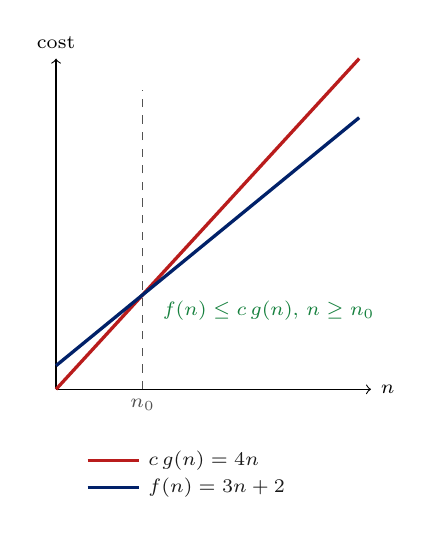
\begin{tikzpicture}[every node/.style={font=\scriptsize}]
    \draw[->] (0,0) -- (4.0,0) node[right] {$n$};
    \draw[->] (0,0) -- (0,4.2) node[above] {cost};
    \draw[very thick, color=negative] (0,0) -- (3.85,4.20);
    \draw[very thick, color=primary-blue] (0,0.30) -- (3.85,3.45);
    \draw[dashed, color=neutral] (1.10,0) -- (1.10,3.8);
    \node[color=neutral] at (1.10,-0.2) {$n_0$};
    \node[color=positive] at (2.7,1.0) {$f(n)\le c\,g(n)$, $n\ge n_0$};
    \draw[very thick, color=negative] (0.4,-0.9) -- (1.05,-0.9);
    \node[color=jet, right] at (1.05,-0.9) {$c\,g(n)=4n$};
    \draw[very thick, color=primary-blue] (0.4,-1.25) -- (1.05,-1.25);
    \node[color=jet, right] at (1.05,-1.25) {$f(n)=3n+2$};
  \end{tikzpicture}
  \caption{Big-$O$ as an upper bound: $f(n)=3n+2$ is eventually at or below
  $c\,g(n)=4n$, for every $n \ge n_0$.}
  \label{fig:bigo}
\end{figure}

\begin{example}[$T(n) = 3n + 2$ is $O(n)$]
Claim: choosing $c = 4$ and $n_0 = 2$ satisfies the definition. Check the
boundary first, at $n = n_0 - 1 = 1$: $3(1) + 2 = 5$, while $4 \cdot 1 = 4$,
and $5 > 4$ --- the inequality \emph{fails} at $n = 1$, which is exactly why
$n_0$ cannot be taken as $0$ or $1$ here. Now check $n = n_0 = 2$:
$3(2) + 2 = 8$, while $4 \cdot 2 = 8$, and $8 \leq 8$ --- the inequality
holds, with equality. For any $n > 2$, the linear term $3n$ grows at the
same rate as $4n$ but $4n$ started with a $1n$ head start built into the
constant $4$ versus $3$, so once the $+2$ has been absorbed at $n=2$ the gap
only widens: $4n - (3n+2) = n - 2 \geq 0$ for all $n \geq 2$. So $3n + 2 \leq
4n$ holds for every $n \geq 2$, confirming $c = 4$, $n_0 = 2$ is a valid
choice, and therefore $T(n) = O(n)$. The exact function was $3n + 2$; the
asymptotic class the analysis reports is simply $O(n)$ --- reading it aloud,
``the running time is of order $n$,'' already throws away the $3$ and the
$2$ as constants that do not change the shape of the growth.
\end{example}

\subsection{Big-Omega: a lower bound}

\begin{definitionbox}{Big-Omega}
$T(n) = \Omega(g(n))$ if there exist constants $c > 0$ and $n_0 \geq 0$ such
that
\[
  T(n) \geq c \cdot g(n) \quad \text{for all } n \geq n_0.
\]
\end{definitionbox}

In words: $T(n)$ grows \emph{at least} as fast as $g(n)$, up to a constant
factor. Where $O$ answers ``at worst, how much work,'' $\Omega$ answers ``at
best, how much work'' --- a guarantee on how \emph{little} the cost can be,
not how much.

\begin{figure}[h]
  \centering
  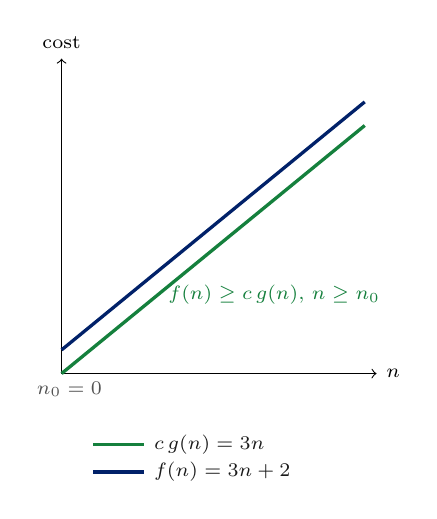
\begin{tikzpicture}[every node/.style={font=\scriptsize}]
    \draw[->] (0,0) -- (4.0,0) node[right] {$n$};
    \draw[->] (0,0) -- (0,4.0) node[above] {cost};
    \draw[very thick, color=positive] (0,0) -- (3.85,3.15);
    \draw[very thick, color=primary-blue] (0,0.30) -- (3.85,3.45);
    \node[color=neutral] at (0.1,-0.2) {$n_0=0$};
    \node[color=positive] at (2.7,1.0) {$f(n)\ge c\,g(n)$, $n\ge n_0$};
    \draw[very thick, color=positive] (0.4,-0.9) -- (1.05,-0.9);
    \node[color=jet, right] at (1.05,-0.9) {$c\,g(n)=3n$};
    \draw[very thick, color=primary-blue] (0.4,-1.25) -- (1.05,-1.25);
    \node[color=jet, right] at (1.05,-1.25) {$f(n)=3n+2$};
  \end{tikzpicture}
  \caption{Big-$\Omega$ as a lower bound: $f(n)=3n+2$ is always at or above
  $c\,g(n)=3n$.}
  \label{fig:bigomega}
\end{figure}

\begin{example}[$T(n) = 3n + 2$ is $\Omega(n)$]
Claim: choosing $c = 3$ and $n_0 = 0$ satisfies the definition. The
inequality to check is $3n + 2 \geq 3n$ for every $n \geq 0$; subtracting
$3n$ from both sides gives $2 \geq 0$, which is true unconditionally, for
every value of $n$. So the inequality holds for \emph{all} $n \geq 0$, and in
particular for all $n \geq n_0 = 0$, confirming $T(n) = \Omega(n)$ with
$c = 3$.
\end{example}

\subsection{Big-Theta: a tight bound}

\begin{definitionbox}{Big-Theta}
$T(n) = \Theta(g(n))$ when $T(n)$ is \emph{both} $O(g(n))$ and $\Omega(g(n))$
--- that is, when $g(n)$ sandwiches $T(n)$ from above and below, each up to
its own constant.
\end{definitionbox}

In words: $T(n)$ grows \emph{exactly} like $g(n)$, up to a constant factor,
in both directions at once. $\Theta$ is the strongest of the three claims,
and should be used only when both bounds genuinely meet.

\begin{figure}[h]
  \centering
  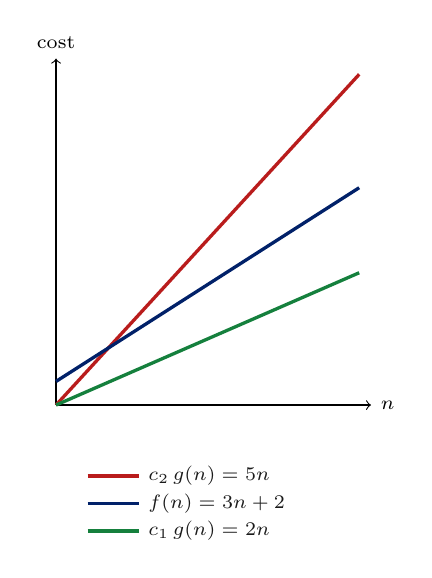
\begin{tikzpicture}[every node/.style={font=\scriptsize}]
    \draw[->] (0,0) -- (4.0,0) node[right] {$n$};
    \draw[->] (0,0) -- (0,4.4) node[above] {cost};
    \draw[very thick, color=negative] (0,0) -- (3.85,4.20);
    \draw[very thick, color=primary-blue] (0,0.30) -- (3.85,2.76);
    \draw[very thick, color=positive] (0,0) -- (3.85,1.68);
    \draw[very thick, color=negative] (0.4,-0.9) -- (1.05,-0.9);
    \node[color=jet, right] at (1.05,-0.9) {$c_2\,g(n)=5n$};
    \draw[very thick, color=primary-blue] (0.4,-1.25) -- (1.05,-1.25);
    \node[color=jet, right] at (1.05,-1.25) {$f(n)=3n+2$};
    \draw[very thick, color=positive] (0.4,-1.6) -- (1.05,-1.6);
    \node[color=jet, right] at (1.05,-1.6) {$c_1\,g(n)=2n$};
  \end{tikzpicture}
  \caption{Big-$\Theta$ as a tight bound: $f(n)=3n+2$ is sandwiched between
  $c_1\,g(n)=2n$ below and $c_2\,g(n)=5n$ above.}
  \label{fig:bigtheta}
\end{figure}

\begin{example}[$T(n) = 3n + 2$ is $\Theta(n)$]
This is where the $O$ and $\Omega$ results above are combined. \textbf{Lower
bound.} Take $c_1 = 2$: the inequality $3n + 2 \geq 2n$ simplifies (subtract
$2n$ from both sides) to $n + 2 \geq 0$, which holds for every $n \geq 0$.
\textbf{Upper bound.} Take $c_2 = 5$: the inequality $3n + 2 \leq 5n$
simplifies (subtract $3n$, then divide by $2$) to $1 \leq n$, so this bound
holds for $n \geq 1$. Combining the two: for every $n \geq 1$, both
$2n \leq 3n + 2$ and $3n + 2 \leq 5n$ hold simultaneously, i.e.\
$2n \leq 3n+2 \leq 5n$ --- exactly the sandwich $\Theta$ requires, with
$c_1 = 2$, $c_2 = 5$, $n_0 = 1$. So $T(n) = 3n+2$ is $\Theta(n)$: it is
bounded below by $2n$ and above by $5n$.
\end{example}

\subsection{The strict siblings: little-o and little-omega}

\begin{definitionbox}{Little-o and little-omega}
$T(n) = o(g(n))$ means $T(n)/g(n) \to 0$ as $n \to \infty$ --- a
\emph{strict} upper bound. $T(n) = \omega(g(n))$ means $T(n)/g(n) \to
\infty$ as $n \to \infty$ --- a \emph{strict} lower bound.
\end{definitionbox}

The strict forms tighten $O$ and $\Omega$ by ruling out the boundary case
where the two functions actually grow at the \emph{same} rate. For example,
$n = o(n^2)$, since $n/n^2 = 1/n \to 0$; but $2n$ is \emph{not} $o(n)$,
since $2n/n = 2$, a nonzero constant, not a ratio tending to $0$. Likewise
$n^2 = \omega(n)$, since $n^2/n = n \to \infty$; but $2n$ is \emph{not}
$\omega(n)$, since $2n/n = 2$ again, not a ratio tending to infinity. These
strict forms are rarely needed in this course; the vast majority of claims
made from here on will use $O$, $\Omega$, or $\Theta$.

\subsection{Reading notation correctly}

A bound must always name its case, or the claim is incomplete. ``Linear
search is $O(n)$'' on its own does not say \emph{in which case} --- best,
worst, or average --- the bound applies, and different cases of the same
algorithm can have entirely different bounds. Correctly stated claims name
both the bound and the case: \good{linear search is $O(n)$ in the worst
case}, and \good{linear search is $\Omega(1)$ in the best case}. Two common
errors to avoid: \bad{``binary search is $O(\log n)$''} states no case at
all, leaving the reader to guess which input the bound describes; and
\bad{``$T(n) = O(n)$, so exactly $n$ steps''} confuses an asymptotic
\emph{class} with an exact \emph{count} --- $O(n)$ describes a whole family
of functions that grow no faster than some constant multiple of $n$, not the
single function ``$n$.'' \key{Pair every complexity claim with the case, and
name the operation being counted.}

\section{Two Searches, Two Costs}
\label{sec:searches}

With the vocabulary of Sections~\ref{sec:counting}--\ref{sec:notation} in
hand, this section applies it to the two searches introduced informally in
Section~\ref{sec:motivation}: the linear scan and the sorted-array jump.

\subsection{Linear search, analysed}

Counting the comparison \texttt{A[i] == key} as before, the three cases
established in Section~\ref{sec:cases} translate directly into asymptotic
classes. The worst case costs $n$ comparisons, i.e.\ $O(n)$ --- exhibited by
the trace where \texttt{key} is absent and every \texttt{A[i]} is examined
exactly once. The best case costs $1$ comparison --- exhibited by
\texttt{key == A[0]}. The average case costs $\frac{n+1}{2}$ comparisons,
which is $\Theta(n)$, since $\frac{n+1}{2}$ is sandwiched between $c_1 n$
and $c_2 n$ for suitable constants (indeed $\frac{n+1}{2} \geq \frac{1}{2}n$
for all $n \geq 0$, and $\frac{n+1}{2} \leq n$ for all $n \geq 1$). Every one
of these three claims names its case explicitly, and each is matched to the
specific input that exhibits it --- exactly the discipline
Section~\ref{sec:notation} insisted on.

\subsection{Binary search needs a sorted table}

Binary search is only \emph{correct} when the array is sorted; this is a
precondition of the algorithm, an invariant that must hold before a single
comparison is made --- not an option to be checked later. The reason is
structural: the sorted order is precisely what makes halving valid. After
one comparison against the middle element, binary search discards an entire
half of the remaining range, trusting that every element in the discarded
half is on the wrong side of \texttt{key}. That trust is only justified when
the array is sorted; on an unsorted array, the middle element's relationship
to its neighbours says nothing about where a target value might sit, so
discarding a whole half can silently discard the very half containing
\texttt{key} --- the algorithm would then report ``not found'' for a key
that is actually present, without any error or warning. Keeping a table
sorted is itself a cost, paid on every insertion, in exchange for the
lookup speed binary search buys once the table is sorted --- a trade-off
this chapter's vocabulary will let us state precisely in
Section~\ref{sec:searches-payoff}. The anti-pattern to guard against, stated
once and worth repeating: never apply binary search without first stating
and checking the sorted precondition.

\begin{example}[Binary search]
\begin{verbatim}
int binary_search(int A[], int n, int key) {
    int lo = 0, hi = n - 1;
    while (lo <= hi) {
        int mid = lo + (hi - lo) / 2;
        if (A[mid] == key) return mid;
        else if (A[mid] < key) lo = mid + 1;
        else                  hi = mid - 1;
    }
    return -1;
}
\end{verbatim}
Each pass compares \texttt{A[mid]} against \texttt{key} and shrinks the
active range \texttt{[lo, hi]} by roughly half: if \texttt{A[mid]} is too
small, the entire lower half (including \texttt{mid}) is discarded by
setting \texttt{lo = mid + 1}; if \texttt{A[mid]} is too large, the entire
upper half is discarded by setting \texttt{hi = mid - 1}. The array
\texttt{A} must already be sorted in ascending order for this discarding
logic to be valid, per the precondition above.
\end{example}

Figure~\ref{fig:halving} shows the array \texttt{A} used in the worked trace
below, with \texttt{lo}, \texttt{mid}, and \texttt{hi} marking the state
after the loop's first pass computes \texttt{mid = lo + (hi - lo) / 2},
landing on index $4$ (value $30$).

\begin{figure}[h]
  \centering
  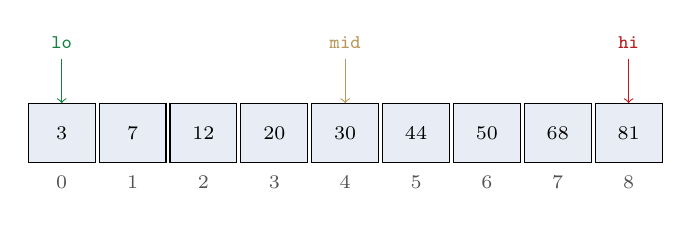
\begin{tikzpicture}[every node/.style={font=\scriptsize}]
    \foreach \i/\v in {0/3,1/7,2/12,3/20,4/30,5/44,6/50,7/68,8/81} {
      \node[draw, minimum width=0.85cm, minimum height=0.75cm, fill=light-bg]
        (\i) at (0.9*\i, 0) {\v};
    }
    \foreach \i in {0,...,8} {
      \node[text=neutral] at (0.9*\i, -0.62) {\i};
    }
    \node[text=positive] (lo) at (0, 1.15) {\texttt{lo}};
    \node[text=primary-gold] (mid) at (0.9*4, 1.15) {\texttt{mid}};
    \node[text=negative] (hi) at (0.9*8, 1.15) {\texttt{hi}};
    \draw[->, color=positive] (lo.south) -- (0.north);
    \draw[->, color=primary-gold] (mid.south) -- (4.north);
    \draw[->, color=negative] (hi.south) -- (8.north);
  \end{tikzpicture}
  \caption{Binary search on \texttt{A = [3, 7, 12, 20, 30, 44, 50, 68, 81]}
  ($n=9$): the first pass's \texttt{lo}, \texttt{mid}, \texttt{hi} pointers.
  Since $30 < 68$, the left half (indices $0$--$4$) is discarded and
  \texttt{lo} jumps to $5$.}
  \label{fig:halving}
\end{figure}

\begin{example}[Binary search trace, \texttt{key = 68}]
Searching the array of Figure~\ref{fig:halving} for \texttt{key = 68},
tracing \texttt{lo}, \texttt{hi}, \texttt{mid}, and the comparison at each
pass, one pass at a time:

\textbf{Pass 1.} \texttt{lo = 0}, \texttt{hi = 8}. Compute
\texttt{mid = 0 + (8 - 0) / 2 = 4}. Compare \texttt{A[4] = 30} against
\texttt{key = 68}: since $30 < 68$, the target must be in the upper half, so
set \texttt{lo = mid + 1 = 5}.

\textbf{Pass 2.} \texttt{lo = 5}, \texttt{hi = 8}. Compute
\texttt{mid = 5 + (8 - 5) / 2 = 5 + 1 = 6}. Compare \texttt{A[6] = 50}
against \texttt{key = 68}: since $50 < 68$, set \texttt{lo = mid + 1 = 7}.

\textbf{Pass 3.} \texttt{lo = 7}, \texttt{hi = 8}. Compute
\texttt{mid = 7 + (8 - 7) / 2 = 7 + 0 = 7} (integer division truncates).
Compare \texttt{A[7] = 68} against \texttt{key = 68}: they are equal, so the
function returns \texttt{mid = 7} immediately.

\begin{center}
\begin{tabular}{ccccc}
\toprule
\textbf{pass} & \texttt{lo} & \texttt{hi} & \texttt{mid} & \texttt{A[mid]} \\
\midrule
1 & 0 & 8 & 4 & $30 < 68$ \\
2 & 5 & 8 & 6 & $50 < 68$ \\
3 & 7 & 8 & 7 & $68 = 68$ --- found \\
\bottomrule
\end{tabular}
\end{center}

Three passes locate \texttt{key = 68} among $n = 9$ values. For comparison,
a linear scan starting from index $0$ would have to check several of the
array's early cells before ever reaching index $7$ where \texttt{68} sits;
in the worst case a linear scan over this same array checks every one of
its $9$ cells. Each binary-search pass discards half of the remaining
interval, and that halving is the entire engine behind the logarithmic
bound derived next.
\end{example}

\subsection{Binary search, analysed}

Each pass halves the active interval \texttt{[lo, hi]}: after $k$ passes, at
most $\lceil n / 2^k \rceil$ elements remain under consideration (this is an
upper bound on the number of surviving elements, consistent with --- though
not identical to --- the specific counts in the trace above, since the trace
is one concrete run and the formula bounds every possible run). The loop
stops as soon as the interval becomes empty, i.e.\ once $\lceil n/2^k
\rceil$ reaches $1$ or below, which happens once $k$ is about $\log_2 n$.
Concretely, for $n = 9$: after $1$ pass at most $\lceil 9/2 \rceil = 5$
elements remain, after $2$ passes at most $\lceil 9/4 \rceil = 3$ remain,
after $3$ passes at most $\lceil 9/8 \rceil = 2$ remain, and after $4$
passes at most $\lceil 9/16 \rceil = 1$ remains --- consistent with the
worked trace needing only $3$ passes to finish (the specific target's
position let it finish slightly before the general bound is exhausted).
\key{Binary search is $O(\log n)$ in the worst case} --- $\log$ here is the
base-$2$ logarithm, but the base is itself only a constant factor, which
asymptotic notation drops regardless of which base is chosen. \key{Binary
search is $\Omega(1)$ in the best case}, exhibited when \texttt{key} sits
exactly at \texttt{A[mid]} on the very first pass.

\begin{example}[A nested loop: checking for duplicates]
A third algorithm worth analysing checks whether the symbol table already
holds the same name twice:
\begin{verbatim}
for (int i = 0; i < n; i++)
    for (int j = i + 1; j < n; j++)
        if (A[i] == A[j])
            return 1;  /* duplicate found */
\end{verbatim}
For a fixed value of the outer index \texttt{i}, the inner loop's index
\texttt{j} runs from \texttt{i + 1} up to \texttt{n - 1}, which is
$n - (i+1) = n - i - 1$ iterations, each performing one comparison
\texttt{A[i] == A[j]}. Summing over every value of \texttt{i} from $0$ to
$n - 2$ (the last value for which the inner loop can run at all) gives the
total comparison count
\[
  T(n) = \sum_{i=0}^{n-2} (n - i - 1).
\]
Substitute $j = n - i - 1$: as $i$ ranges over $0, 1, \dots, n-2$, the new
index $j$ ranges over $n-1, n-2, \dots, 1$ --- the same set of values,
counted in the opposite order. So the sum is exactly
\[
  \sum_{j=1}^{n-1} j = \frac{(n-1)n}{2} = \frac{n(n-1)}{2},
\]
using the same closed form for a sum of consecutive integers derived in
Section~\ref{sec:cases}. Expanding, $\frac{n(n-1)}{2} = \frac{n^2 - n}{2}$,
whose dominant term is $\frac{1}{2}n^2$ --- a constant multiple of $n^2$, so
$T(n) = \Theta(n^2)$: since the loop as written always runs to completion
unless a duplicate is actually encountered and triggers the early
\texttt{return 1}, the full double loop --- and hence the $\Theta(n^2)$ count
--- describes every run in which no duplicate exists to trigger an early
exit.
\end{example}

\begin{table}[h]
\centering
\begin{tabular}{rrrrr}
\toprule
$n$ & $\log_2 n$ & $n$ & $n \log_2 n$ & $n^2$ \\
\midrule
$10$   & $\approx 3$  & $10$   & $\approx 33$        & $10^2$ \\
$10^3$ & $\approx 10$ & $10^3$ & $\approx 10^4$       & $10^6$ \\
$10^6$ & $\approx 20$ & $10^6$ & $\approx 2\cdot10^7$ & $10^{12}$ \\
\bottomrule
\end{tabular}
\caption{The orders of growth from Table~\ref{tab:orders}, evaluated at
concrete input sizes.}
\label{tab:numbers}
\end{table}

Table~\ref{tab:numbers} makes the shape of these growth rates concrete: as
$n$ grows from $10$ to a million, $\log_2 n$ barely moves --- from about $3$
to about $20$ --- while $n^2$ explodes from $100$ to a trillion. This is the
practical difference between a search that remains usable as the data grows
and one that does not.

\subsection{The symbol table payoff}
\label{sec:searches-payoff}

Returning to the running example one more time: the calculator's identifier
lookup, analysed as $n$ grows, now has a precise trade-off attached to each
of its three possible homes. As an \key{unsorted list} (the implementation
Week 6 will build), lookup costs $O(n)$ in the worst case --- the whole
table may need scanning. As a \key{sorted array}, lookup costs $O(\log n)$
in the worst case via binary search --- but keeping the array sorted costs
something on every insertion, since a new identifier may need to be slotted
into the middle of an already-sorted range. As a \key{hash table} (the
implementation Week 10 will build), lookup costs $O(1)$ \emph{expected} ---
the entire reason a hash table will eventually be worth building. This
chapter supplies the vocabulary that makes this three-way trade-off
precise; Weeks 6 and 10 will act on it by actually building the list and the
hash table and confirming the bounds empirically.

\section{Space Complexity}
\label{sec:space}

\begin{definitionbox}{Space complexity $S(n)$}
$S(n)$ is the amount of memory an algorithm uses \emph{beyond} its input ---
its \emph{auxiliary} space --- as a function of $n$.
\end{definitionbox}

Two components make up an algorithm's total memory use: \key{input space},
the $n$ elements of the input itself, counted separately since every
algorithm operating on an array of size $n$ trivially needs at least that
much memory to hold the array; and \key{auxiliary space}, the \emph{extra}
working memory the algorithm needs beyond the input --- extra local
variables, temporary arrays, or recursion stack frames. $S(n)$ is stated in
exactly the same asymptotic classes as $T(n)$: $O(1)$, $O(\log n)$, $O(n)$,
and so on. The two are separated because ``this algorithm uses $n$ memory
cells'' is an uninteresting observation when the input already occupies $n$
cells regardless of the algorithm; the auxiliary space is the number that
actually distinguishes one algorithm's memory footprint from another's.

Both of this chapter's search algorithms keep only a small, fixed handful
of local variables, independent of $n$. \texttt{linear\_search} uses one
index variable \texttt{i}: auxiliary space $O(1)$. \texttt{binary\_search}
uses three index variables, \texttt{lo}, \texttt{hi}, and \texttt{mid}:
auxiliary space $O(1)$ as well, since three variables is still a constant,
regardless of how large $n$ is. A \emph{recursive} implementation of binary
search, by contrast, would use $O(\log n)$ auxiliary space --- not because
the recursive version stores more data explicitly, but because each
recursive call adds one more stack frame (Week 1's stack-frame picture,
reused here), and the recursion depth for binary search is itself $O(\log
n)$, matching the number of passes derived in
Section~\ref{sec:searches}. $O(1)$ auxiliary space is a property this course
will price carefully later: Week 9 compares in-place sorting algorithms
against mergesort precisely on this axis. The underlying intuition is
Week 1's: each variable, wherever it lives --- stack or heap --- occupies
one cell, and counting cells is exactly what $S(n)$ does.

\section{Common Mistakes and What Comes Next}
\label{sec:mistakes}

Three mistakes recur often enough with this material that they are worth
naming explicitly, so that each can be caught in your own writing before it
becomes a habit. \bad{Treating $T(n) = O(n)$ as an exact count}: $O(n)$
names a whole \emph{class} of functions that grow no faster than some
constant multiple of $n$; it is not a claim that the algorithm performs
exactly $n$ steps. \bad{Stating a bound with no case}: ``$O(n)$'' by itself,
with no mention of best, worst, or average, is an unfalsifiable claim,
because the same algorithm can have entirely different bounds in different
cases, as Section~\ref{sec:searches} showed for linear search. \bad{Mixing
up $O$ and $\Theta$}: $O$ is only an upper bound, possibly loose; only
$\Theta$ asserts that the growth rate matches \emph{exactly}, from both
above and below. The habit that avoids all three mistakes at once: name the
operation being counted, give the bound, state the case, and point to the
specific input that exhibits it --- exactly the pattern followed by every
worked example in this chapter.

Next week turns to Arrays and the Stack ADT --- the first data structure
this course will analyse end to end, using precisely the cost-model
vocabulary just built here: a contract (Week 1's ADT idea), an
implementation, and now a cost, stated with its case.

\subsection*{Exercises}

\begin{enumerate}
  \item The calculator's symbol table doubles in size, from $n$ to $2n$
    names. For each of the following operations, state --- and justify from
    its asymptotic class --- roughly how much more expensive the operation
    becomes: (a) a linear scan of the table; (b) a binary search of the
    table (assume it is kept sorted); (c) the nested-loop duplicate check of
    Section~\ref{sec:searches}.
  \item Trace \texttt{linear\_search} comparison by comparison on
    \texttt{A = [5, 15, 25, 35]} (so $n = 4$) searching for
    \texttt{key = 25}. State the number of comparisons performed, and say
    whether this run exhibits the best case, the worst case, or neither.
  \item Show that $T(n) = 5n + 10$ is $O(n)$ by exhibiting valid constants
    $c$ and $n_0$ and verifying the defining inequality holds for all
    $n \geq n_0$.
  \item Show that $T(n) = 2n^2 + 3n$ is $\Theta(n^2)$ by exhibiting valid
    constants $c_1$, $c_2$, and $n_0$ for both the lower and the upper
    bound, and verifying each inequality.
  \item Trace \texttt{binary\_search} on the same array used in
    Section~\ref{sec:searches}, \texttt{A = [3, 7, 12, 20, 30, 44, 50, 68,
    81]} ($n = 9$), this time searching for \texttt{key = 20}. Produce a
    pass-by-pass table of \texttt{lo}, \texttt{hi}, \texttt{mid}, and the
    comparison result, and state how many passes the search takes.
\end{enumerate}

\subsection*{Solutions}

\begingroup\small
\begin{enumerate}
  \item \textbf{Doubling the table:}
    \begin{itemize}
      \item[(a)] A linear scan's worst/average-case cost is $\Theta(n)$.
        Doubling $n$ to $2n$ scales the cost by the ratio $T(2n)/T(n) =
        2n/n = 2$: the linear scan roughly \emph{doubles} in cost.
      \item[(b)] A binary search's worst-case cost is $\Theta(\log n)$.
        Doubling $n$ changes the cost from $\log_2 n$ to
        $\log_2(2n) = \log_2 2 + \log_2 n = 1 + \log_2 n$: doubling the
        table costs exactly \emph{one extra pass}, regardless of how large
        $n$ already was.
      \item[(c)] The nested-loop duplicate check's cost is $\Theta(n^2)$.
        Doubling $n$ changes the cost by the ratio $T(2n)/T(n) =
        (2n)^2/n^2 = 4n^2/n^2 = 4$: the duplicate check becomes
        \emph{four times} as expensive.
    \end{itemize}
    These three ratios --- doubles, one extra pass, four times --- are
    exactly what the asymptotic classes $\Theta(n)$, $\Theta(\log n)$, and
    $\Theta(n^2)$ predict, and are the entire point of building the
    vocabulary this chapter introduces: it lets these predictions be made
    \emph{before} either implementation is built or timed.
  \item \textbf{Trace on \texttt{A = [5, 15, 25, 35]}, \texttt{key = 25}:}
    compare \texttt{A[0] = 5} against $25$ ($5 \ne 25$, comparison $1$);
    compare \texttt{A[1] = 15} against $25$ ($15 \ne 25$, comparison $2$);
    compare \texttt{A[2] = 25} against $25$ ($25 = 25$, comparison $3$,
    match found, return index $2$). The search performs $3$ comparisons.
    For $n = 4$ the best case would cost $1$ comparison and the worst case
    would cost $4$; this run costs $3$, so it exhibits neither the best nor
    the worst case --- it lands between the two, consistent with the
    average-case formula $\frac{n+1}{2} = \frac{5}{2} = 2.5$ from
    Section~\ref{sec:cases} (individual runs vary around that expected
    value; this one happens to cost slightly more than the average).
  \item \textbf{$T(n) = 5n + 10$ is $O(n)$:} choose $c = 6$ and $n_0 = 10$.
    The inequality $5n + 10 \leq 6n$ simplifies (subtract $5n$ from both
    sides) to $10 \leq n$, which is exactly the condition $n \geq n_0 = 10$.
    Checking the boundary at $n = 10$: $5(10) + 10 = 60$, and $6(10) = 60$,
    so $60 \leq 60$ holds with equality. For any $n > 10$ the gap
    $6n - (5n+10) = n - 10 > 0$ only grows, so the inequality continues to
    hold. Hence $T(n) = 5n + 10$ is $O(n)$ with $c = 6$, $n_0 = 10$. (Other
    valid choices exist too --- e.g.\ $c = 15$, $n_0 = 1$ also works, since
    $O$ only requires \emph{some} valid $c$ and $n_0$ to exist, not a unique
    pair.)
  \item \textbf{$T(n) = 2n^2 + 3n$ is $\Theta(n^2)$:} \textbf{lower bound},
    take $c_1 = 2$: the inequality $2n^2 + 3n \geq 2n^2$ simplifies (subtract
    $2n^2$ from both sides) to $3n \geq 0$, true for every $n \geq 0$, so
    this bound holds with $n_0 = 0$. \textbf{Upper bound}, take $c_2 = 5$:
    the inequality $2n^2 + 3n \leq 5n^2$ simplifies (subtract $2n^2$, then
    divide by $3$) to $n \leq n^2$, which holds exactly when $n \geq 1$.
    Combining: for every $n \geq 1$, $2n^2 \leq 2n^2 + 3n \leq 5n^2$ holds
    simultaneously, which is the $\Theta$ sandwich with $c_1 = 2$,
    $c_2 = 5$, $n_0 = 1$. Hence $T(n) = 2n^2 + 3n$ is $\Theta(n^2)$.
  \item \textbf{Binary search trace, \texttt{key = 20}, on
    \texttt{A = [3, 7, 12, 20, 30, 44, 50, 68, 81]} ($n = 9$):}
    \begin{center}
    \begin{tabular}{ccccc}
    \toprule
    \textbf{pass} & \texttt{lo} & \texttt{hi} & \texttt{mid} & \texttt{A[mid]} \\
    \midrule
    1 & 0 & 8 & 4 & $30 > 20$ \\
    2 & 0 & 3 & 1 & $7 < 20$ \\
    3 & 2 & 3 & 2 & $12 < 20$ \\
    4 & 3 & 3 & 3 & $20 = 20$ --- found \\
    \bottomrule
    \end{tabular}
    \end{center}
    Step by step: pass $1$ starts at \texttt{lo=0}, \texttt{hi=8}, so
    \texttt{mid = 0 + (8-0)/2 = 4}; \texttt{A[4] = 30 > 20}, so
    \texttt{hi = mid - 1 = 3}. Pass $2$: \texttt{lo=0}, \texttt{hi=3}, so
    \texttt{mid = 0 + (3-0)/2 = 1}; \texttt{A[1] = 7 < 20}, so
    \texttt{lo = mid + 1 = 2}. Pass $3$: \texttt{lo=2}, \texttt{hi=3}, so
    \texttt{mid = 2 + (3-2)/2 = 2}; \texttt{A[2] = 12 < 20}, so
    \texttt{lo = mid + 1 = 3}. Pass $4$: \texttt{lo=3}, \texttt{hi=3}, so
    \texttt{mid = 3 + (3-3)/2 = 3}; \texttt{A[3] = 20 = 20}, found, return
    \texttt{mid = 3}. The search takes $4$ passes --- one more than the
    $3$-pass trace for \texttt{key = 68} in Section~\ref{sec:searches},
    since $\lceil \log_2 9 \rceil = 4$ is the maximum number of passes
    binary search can take on this array, and this particular target
    happens to require that maximum.
\end{enumerate}
\endgroup

\subsection*{Summary}

\begin{itemize}
  \item \key{Cost model}: count one well-chosen basic operation as a
    function of $n$, giving the exact cost function $T(n)$; compress that
    count into an asymptotic class; always state which case (best, worst,
    average) the count describes.
  \item \key{$T(n)$} is the exact running-time cost function;
    \key{$S(n)$} is the auxiliary space complexity --- memory used beyond
    the input itself, as a function of $n$.
  \item \key{Asymptotic classes}: $O$ (upper bound), $\Omega$ (lower bound),
    $\Theta$ (tight bound, both at once), with the strict forms $o$ and
    $\omega$ available when the gap must be shown to be more than a
    constant factor.
  \item \key{Cases} --- best, worst, average --- are a property of the
    \emph{input}; a bound is a property of the \emph{function}. The two are
    orthogonal and must always be paired, never confused.
  \item \key{Our two searches}: linear search is $O(n)$ in the worst case
    ($\Theta(n)$ on average, $\Omega(1)$ best case); binary search (on a
    sorted array) is $O(\log n)$ in the worst case ($\Omega(1)$ best case);
    a nested-loop duplicate check is $\Theta(n^2)$. Both search algorithms
    use $O(1)$ auxiliary space; a recursive binary search would use
    $O(\log n)$ stack frames instead.
  \item Three habits avoid the recurring mistakes: never treat $O(n)$ as an
    exact step count, never state a bound without its case, and never
    substitute $O$ for $\Theta$ when the growth rate is actually tight in
    both directions.
\end{itemize}

\bibliography{../../Bibliography_base}
\bibliographystyle{plain}

\end{document}
